\documentclass[]{interact}

\usepackage{epstopdf}
\usepackage{subfigure}
\usepackage{booktabs}
\usepackage{graphicx}
\usepackage{natbib}
\usepackage{longtable}
\usepackage{url}
\bibpunct[, ]{(}{)}{,}{a}{}{,}
\renewcommand\bibfont{\fontsize{10}{12}\selectfont}

\begin{document}

\articletype{ARTICLE}

\title{Grounded Workflow Specifications for Reliable LLM-GIS Copilots: A Local-Ollama Benchmark}

\author{
\name{Nguyen The-Vinh\textsuperscript{a}\thanks{CONTACT Nguyen The-Vinh. Email: vinhnt@ictu.edu.vn} and Nguyen Kim-Son\textsuperscript{a}}
\affil{\textsuperscript{a}Thai Nguyen University of Information and Communication Technology, Thai Nguyen, Vietnam}
}

\maketitle

\begin{abstract}
Large language models are increasingly used as GIS copilots, but free-form code generation makes it difficult to separate planning errors, library syntax errors, data hallucination, coordinate-reference-system mistakes, and cartographic artifact failures. This paper introduces a workflow-specification benchmark for evaluating LLM-GIS planning before code execution. Instead of asking models to write Python scripts directly, the benchmark asks local Ollama models to produce structured JSON workflow contracts for GIS tasks under three prompting modes: task-only planning, metadata-grounded planning, and GeoGuard-style planning with validation rules. The full experiment evaluates twelve locally installed models over 30 GIS workflow tasks and three modes, yielding 1080 attempted specifications across buffer, overlay, point-count join, raster clip, zonal statistics, and choropleth-export task families. Grounding changes model behavior substantially. Mean data validity rises from 0.053 in task-only mode to 0.761 in grounded mode, weighted hallucination risk falls from 0.522 to 0.277, and mean plan reliability score rises from 0.547 to 0.751. Adding GeoGuard-style validation rules produces the strongest coordinate-reference-system gains, raising mean CRS planning from 0.674 in grounded mode to 0.774 and reducing CRS-weak cases from 89 to 39 out of 360 tasks. Data-invalid failures fall from 249 in task-only mode to 31 in grounded mode and 25 in GeoGuard mode. The strongest GeoGuard scores are achieved by qwen2.5-coder:3b, gemma3:4b, qwen2.5-coder:14b, qwen2.5-coder:7b, qwen2.5-coder:32b, and deepseek-coder:6.7b, all above 0.93 PRS. In contrast, qwen3:4b fails the strict JSON-contract protocol across the full panel. The contribution is a reproducible benchmark design for evaluating LLM-GIS copilots at the workflow-contract level, before downstream code execution and map rendering are attempted.
\end{abstract}

\begin{keywords}
GIS copilot; large language models; GeoAI; workflow specification; geospatial hallucination; cartographic reliability
\end{keywords}

\section{Introduction}

LLM-based GIS assistants are often evaluated as code generators. A user asks for a buffer, an overlay, a spatial join, a raster clip, or a map, and the model returns a script. This end-to-end setting is realistic, but it is also diagnostically noisy. A failed script may reflect a poor spatial plan, a wrong field name, a hallucinated dataset, an invalid coordinate-reference-system strategy, a missing package import, a changed library API, or a weak map-rendering choice. Conversely, an executable script may still be cartographically unreliable if it uses an inappropriate CRS, silently drops fields, renders an incomplete legend, or produces a map artifact that cannot support the user's geographic question. The problem is therefore not only whether LLMs can write GIS code, but whether they can formulate reliable GIS workflow contracts.

This paper develops a benchmark for that earlier planning layer. Rather than asking a model to write free-form Python, the benchmark asks it to return one structured JSON object that specifies the operation, input layers, parameters, output file, required fields, validation checks, and short rationale for a GIS task. The benchmark then scores the plan itself: whether the JSON is parseable, whether the operation is allowed, whether the referenced layers and fields exist, whether the CRS plan is appropriate, whether required output fields are preserved or created, whether map-export tasks include cartographic elements, and whether the requested output filename is obeyed. This framing treats LLM-GIS reliability as a workflow-contract problem before it becomes a software-execution problem.

The motivation is cartographic as much as computational. Geographic information systems are not generic programming environments; they require explicit attention to spatial reference, topology, schema, measurement, scale, and visual communication \citep{Goodchild_1992,Janowicz_2019,Roth_2013,Roth_2015}. A language model that can produce fluent code may still invent layer names, assume nonexistent attributes, buffer in geographic coordinates, or create a map without a readable legend. These are not superficial errors. They can change the geographic meaning of an analysis or the interpretation of a map. Prior code-generation research has shown the value of systematic benchmarks for language-to-code systems \citep{Li_2022,Xu_2022,Du_2024,Ni_2024,Jiang_2026}, but GIS copilots require additional geospatial validity criteria.

The paper's core claim is that structured workflow specifications provide a useful middle layer between natural-language GIS requests and executable code. This middle layer makes the model's assumptions inspectable and creates a place where metadata grounding, tool schemas, validation rules, and reflection can act before code execution. It also allows local models to be compared under a strict contract without requiring every model to solve all Python, GeoPandas, Rasterio, and cartographic-rendering details at once. The benchmark therefore asks a narrower but important question: when given a natural-language GIS task, can a local LLM produce a valid, grounded, and geospatially faithful workflow specification?

The experiment reported here is a full planning benchmark rather than a single pilot prompt. It covers twelve locally installed Ollama models, three prompting modes, and all 30 tasks in the workflow-specification suite. The resulting 1080 attempted specifications allow the paper to compare model families, prompting regimes, task categories, and failure types under one uniform contract.

\section{Related Work}

\subsection{LLMs for code and workflow generation}

Modern language models can generate executable code, solve programming problems, and assist software repair, but their reliability varies with task structure, context, and evaluation protocol \citep{Li_2022,Xu_2022,Du_2024,Ni_2024,Jiang_2026}. Software-engineering work also shows that repair and validation loops can convert some failed outputs into usable artifacts, while leaving difficult semantic failures unresolved \citep{Gazzola_2019,Monperrus_2018,Le_Goues_2012}. These lessons transfer naturally to GIS, where a script must satisfy both software and spatial contracts.

However, GIS workflows add constraints that are not central in ordinary programming benchmarks. A valid spatial operation depends on layer existence, field schema, geometry type, CRS compatibility, measurement units, raster-vector alignment, and output semantics. A model that writes syntactically valid code can still produce an invalid spatial analysis. This motivates a workflow-specification benchmark: the model must expose the intended operation and parameters before any deterministic executor or code generator runs.

\subsection{GeoAI, cartographic reliability, and map contracts}

GeoAI research emphasizes that spatially explicit AI systems must account for geographic context, spatial dependence, scale, and domain constraints \citep{Janowicz_2019,Zhu_2017,Ma_2019,Kang_2024}. Cartographic research similarly treats maps as designed representations rather than neutral images \citep{Harley_1989,Roth_2013,Roth_2015}. These literatures imply that LLM-GIS evaluation should not stop at generic code success. The generated workflow must preserve geographic meaning.

Recent generative-cartography and LLM-mapmaking studies explore text-to-map generation, LLM-assisted thematic mapping, map style transfer, and cartographic agents \citep{Zhang_2024_MapGPT,Yang_2025_MapColorAI,Zhang_2025_MapGenerator,PannoonNetek_2025_Choropleth,Wang_2025_CartoAgent}. These systems make map production more accessible, but they also amplify the need for explicit validation. If an LLM invents a field, uses the wrong CRS, or produces a map with weak symbology, the artifact can appear plausible while failing its analytic or communicative purpose.

\subsection{Grounding and validation}

Metadata grounding and tool constraints are a practical response to hallucination. Instead of letting a model infer what data might exist, the prompt can provide a data profile and a limited operation schema. This resembles datasheet and model-card thinking in machine-learning documentation: system behavior should be evaluated against declared data and operating conditions \citep{Gebru2021Datasheets,Mitchell2019ModelCards}. In this benchmark, grounding is not a vague prompt-engineering technique; it is an experimentally varied condition. The same model receives either the task alone, the task plus known data/tool metadata, or the task plus metadata and GeoGuard-style validation rules.

\section{Benchmark Design}

\subsection{Task suite}

The benchmark contains 30 natural-language GIS tasks. The tasks are organized into six workflow categories: buffer service areas, overlay intersections, point-count joins, raster clipping, zonal statistics, and choropleth export. The task suite requires hospital-point buffers, clipping to a study boundary, safe metric buffering, flood-zone overlay, school and hospital point-count joins, raster clipping with CRS alignment, zonal temperature statistics, and map export with title, legend, classification, color ramp, and source-note requirements.

The task suite is intentionally contract-oriented. Each task specifies the expected operation type, required output filename, required fields, and natural-language prompt. This allows the scorer to compare the model's workflow specification with an explicit artifact contract rather than relying on a subjective judgment of whether the response ``looks reasonable.'' The 30-task design also prevents the benchmark from being driven by one easy operation type: vector overlays, raster alignment, derived-field schemas, and cartographic map exports produce distinct failure patterns.

Figure~\ref{fig:geo-task-suite} illustrates the kinds of map artifacts implied by the task contracts. The important point is that the benchmark is not asking for generic JSON: each specification must preserve enough geospatial information to support a concrete buffer, overlay, raster, zonal-statistics, or map-export artifact.

\begin{figure}[htbp]
\centering
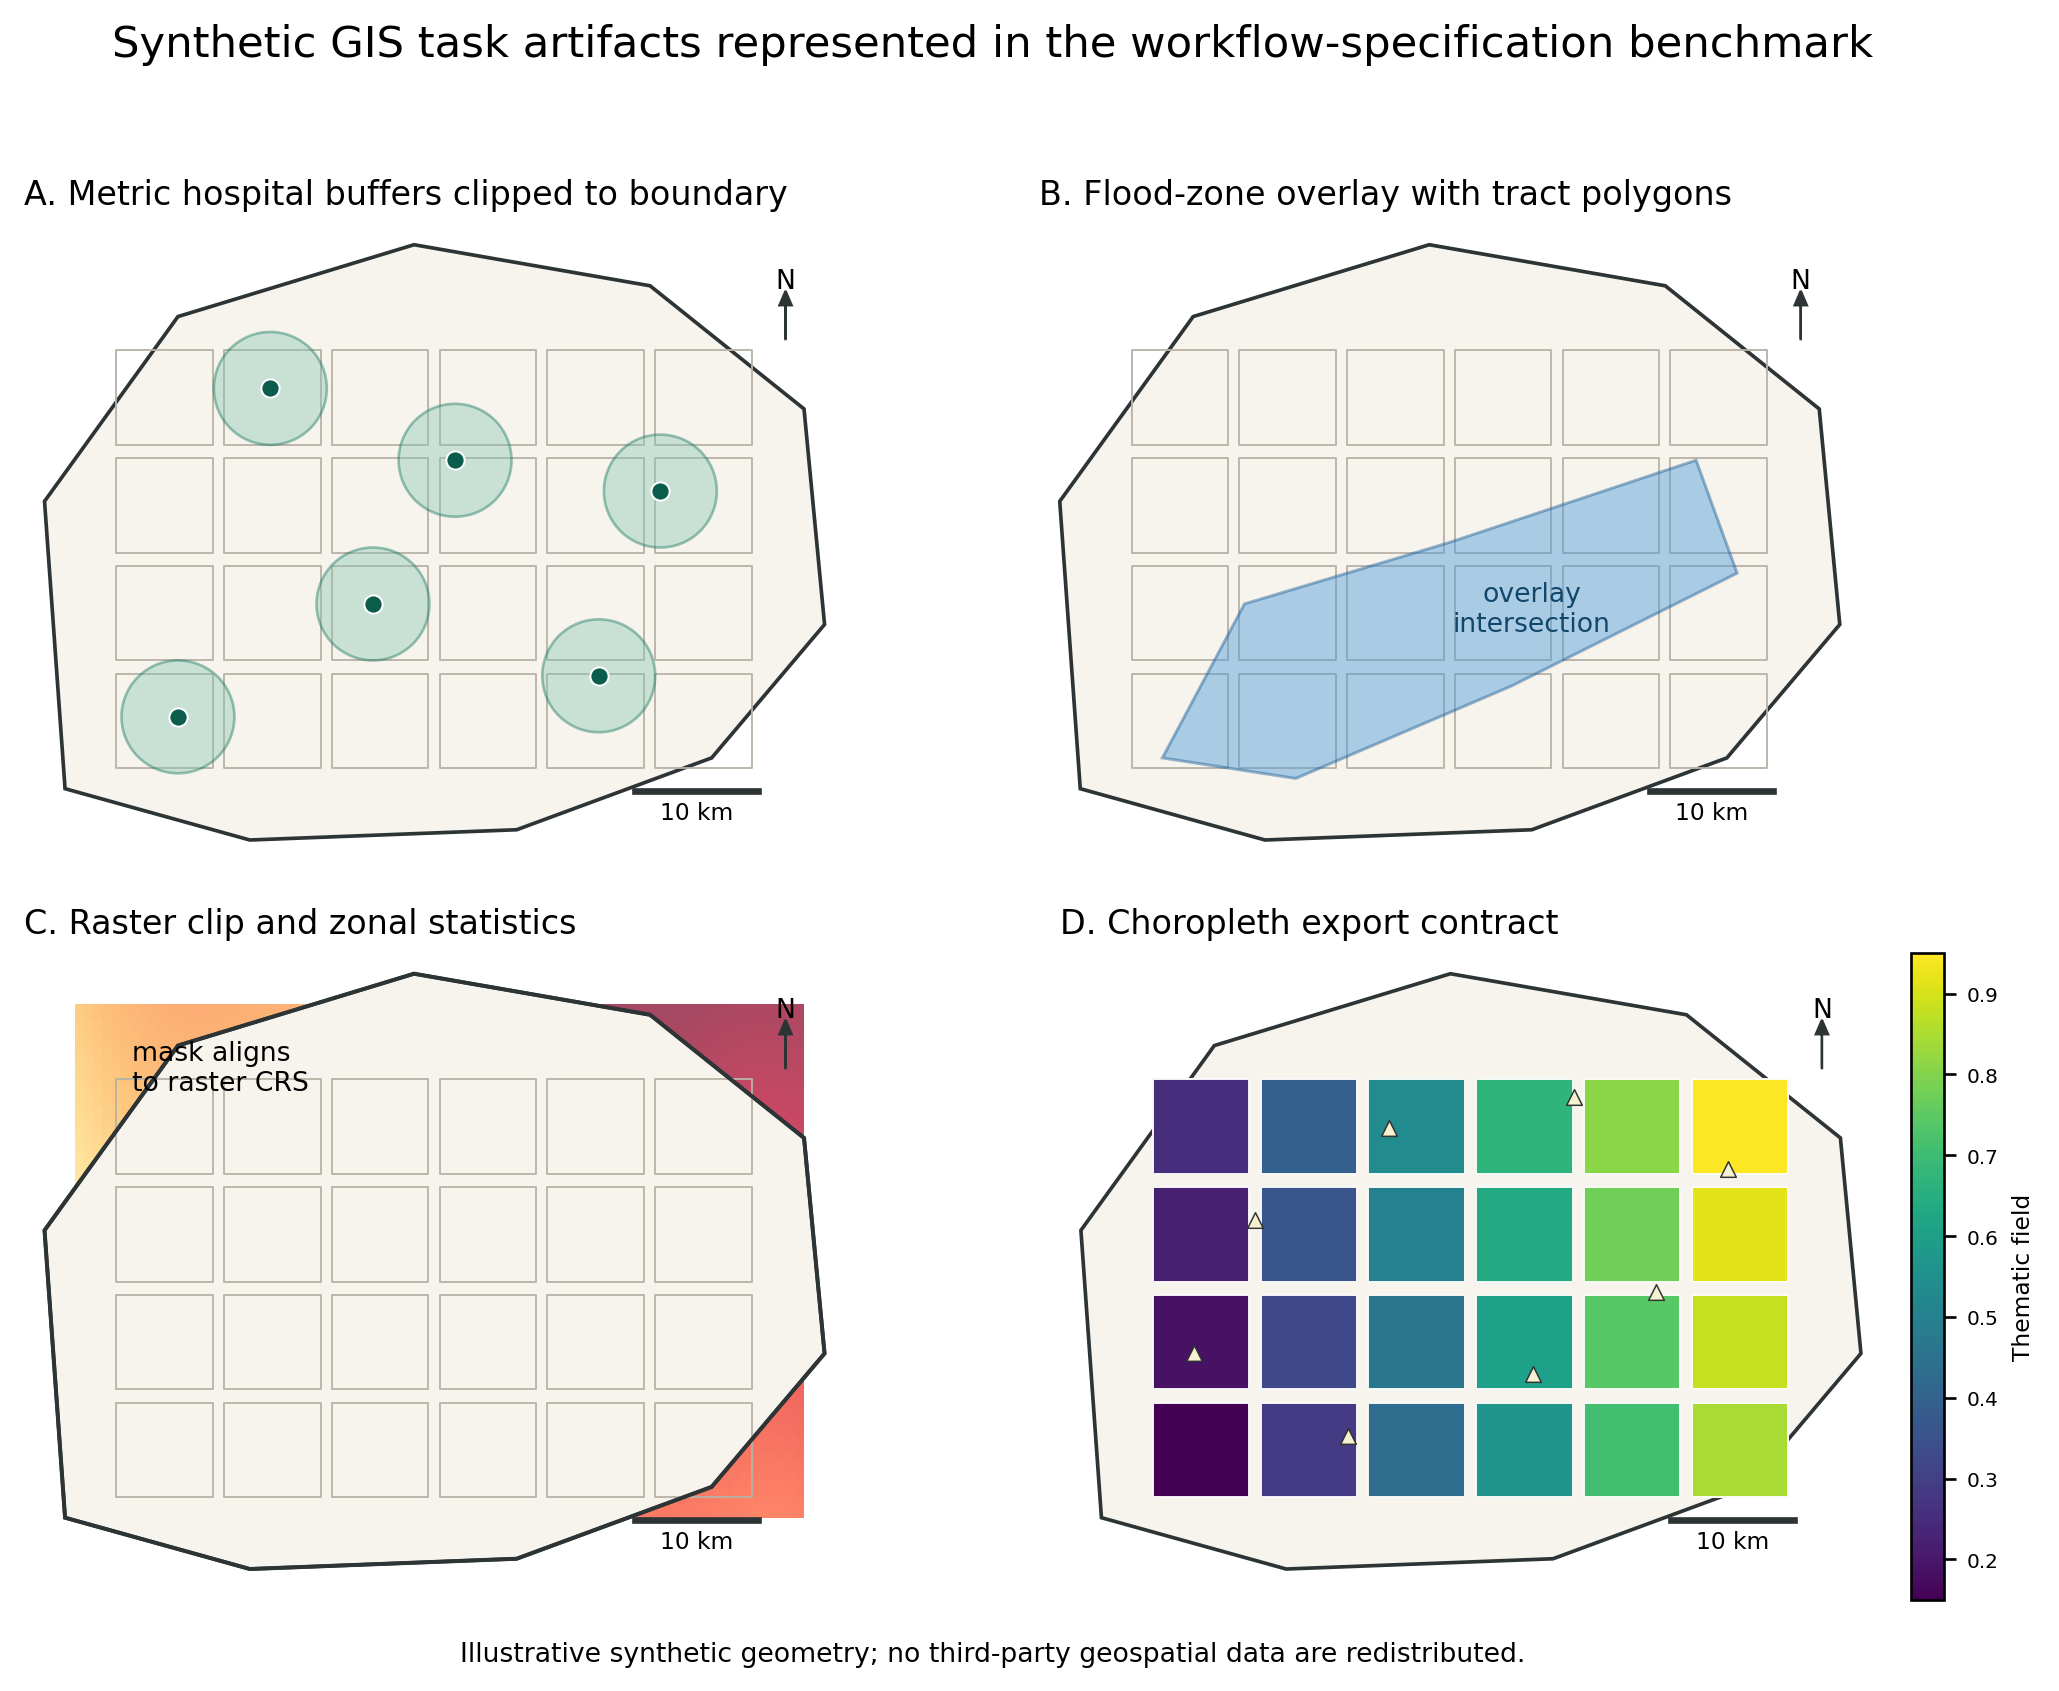
\includegraphics[width=0.98\textwidth]{figures/geo_task_suite_map_examples.png}
\caption{Synthetic GIS artifacts represented by the workflow-specification benchmark. The panels illustrate the geospatial operations that the JSON contracts must describe: metric hospital buffers clipped to a study boundary, flood-zone overlay with tract polygons, raster clipping and zonal statistics, and choropleth export with a thematic field and legend. The geometry is synthetic and is used only to visualize benchmark task semantics.}
\label{fig:geo-task-suite}
\end{figure}

Figure~\ref{fig:geo-operation-gallery} expands this view by showing one map-level example for each operation family. The gallery makes the diagnostic role of the task suite explicit: buffer tasks test distance and projection, overlay tasks test geometry interaction, point-count tasks test spatial aggregation, raster tasks test mask alignment, zonal tasks test raster-vector summaries, and choropleth tasks test cartographic output.

\begin{figure}[htbp]
\centering
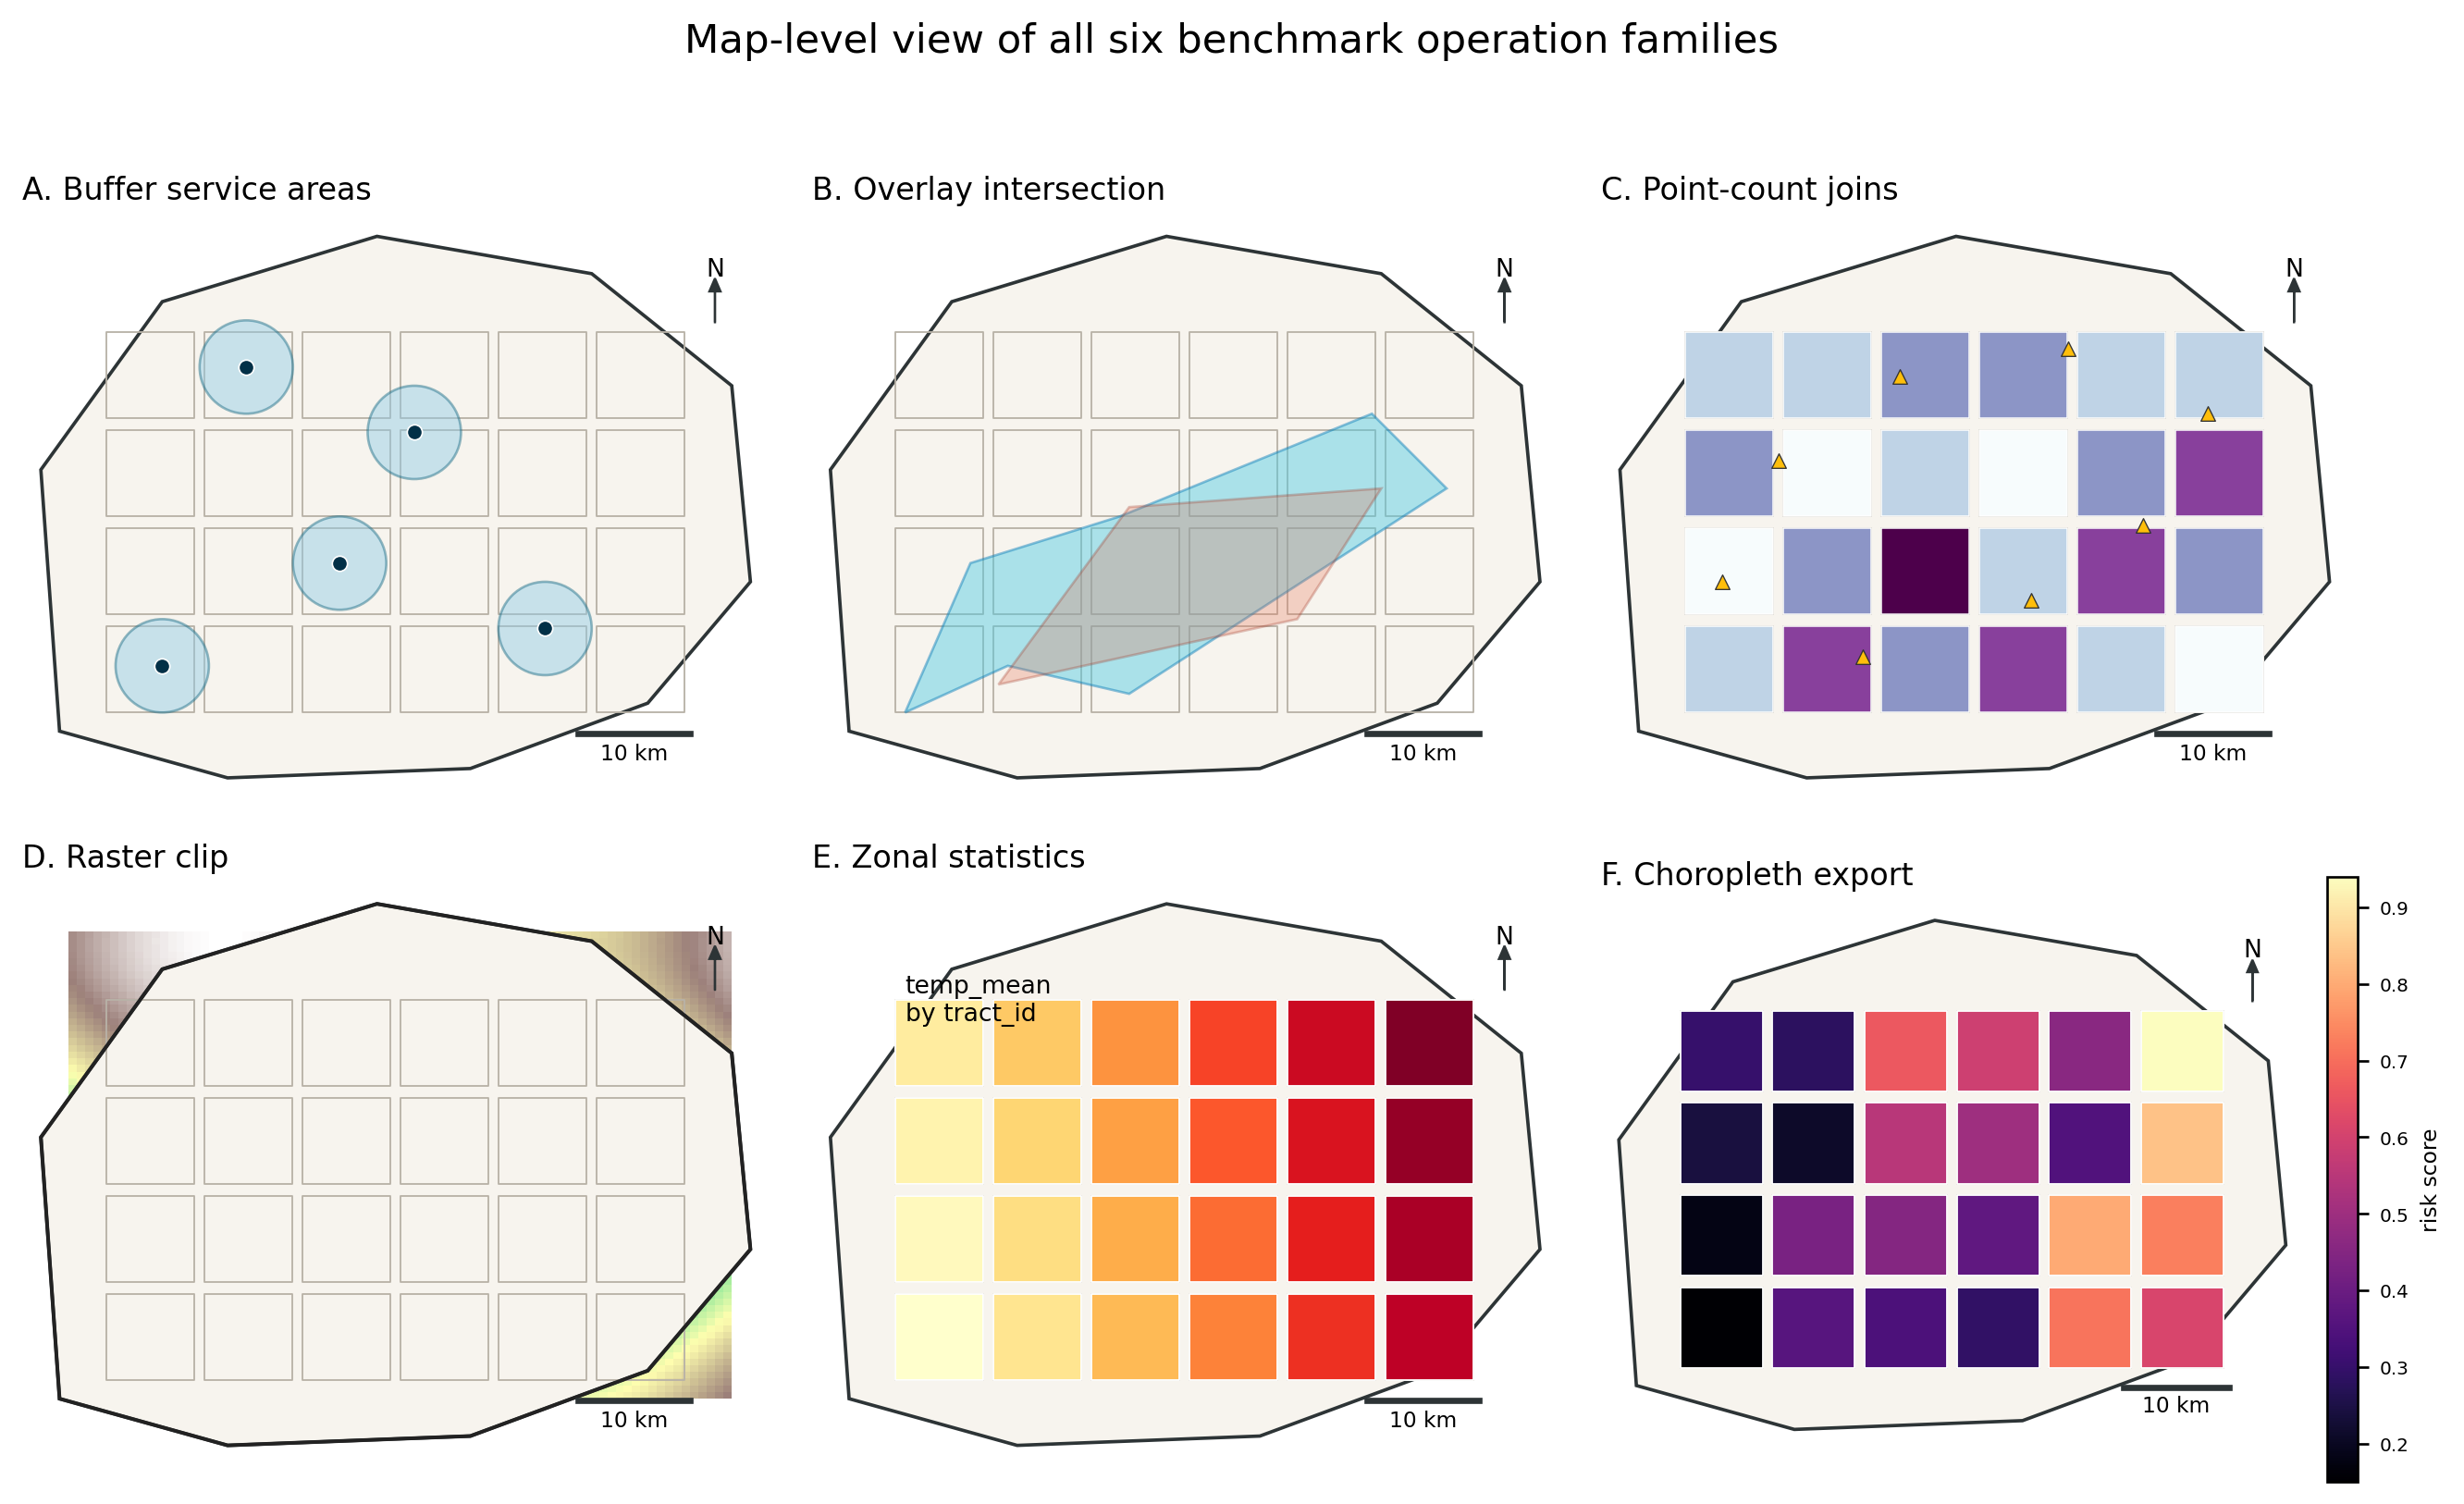
\includegraphics[width=0.98\textwidth]{figures/geo_operation_family_gallery.png}
\caption{Map-level gallery of the six benchmark operation families. The panels make explicit that the benchmark is not only a JSON-format task: it covers vector buffering, overlay, point-in-polygon aggregation, raster masking, zonal statistics, and choropleth map export.}
\label{fig:geo-operation-gallery}
\end{figure}

Figure~\ref{fig:geo-task-family} summarizes the same design at the family level. The six families are intentionally balanced as probes rather than treated as one homogeneous GIS task class.

\begin{figure}[htbp]
\centering
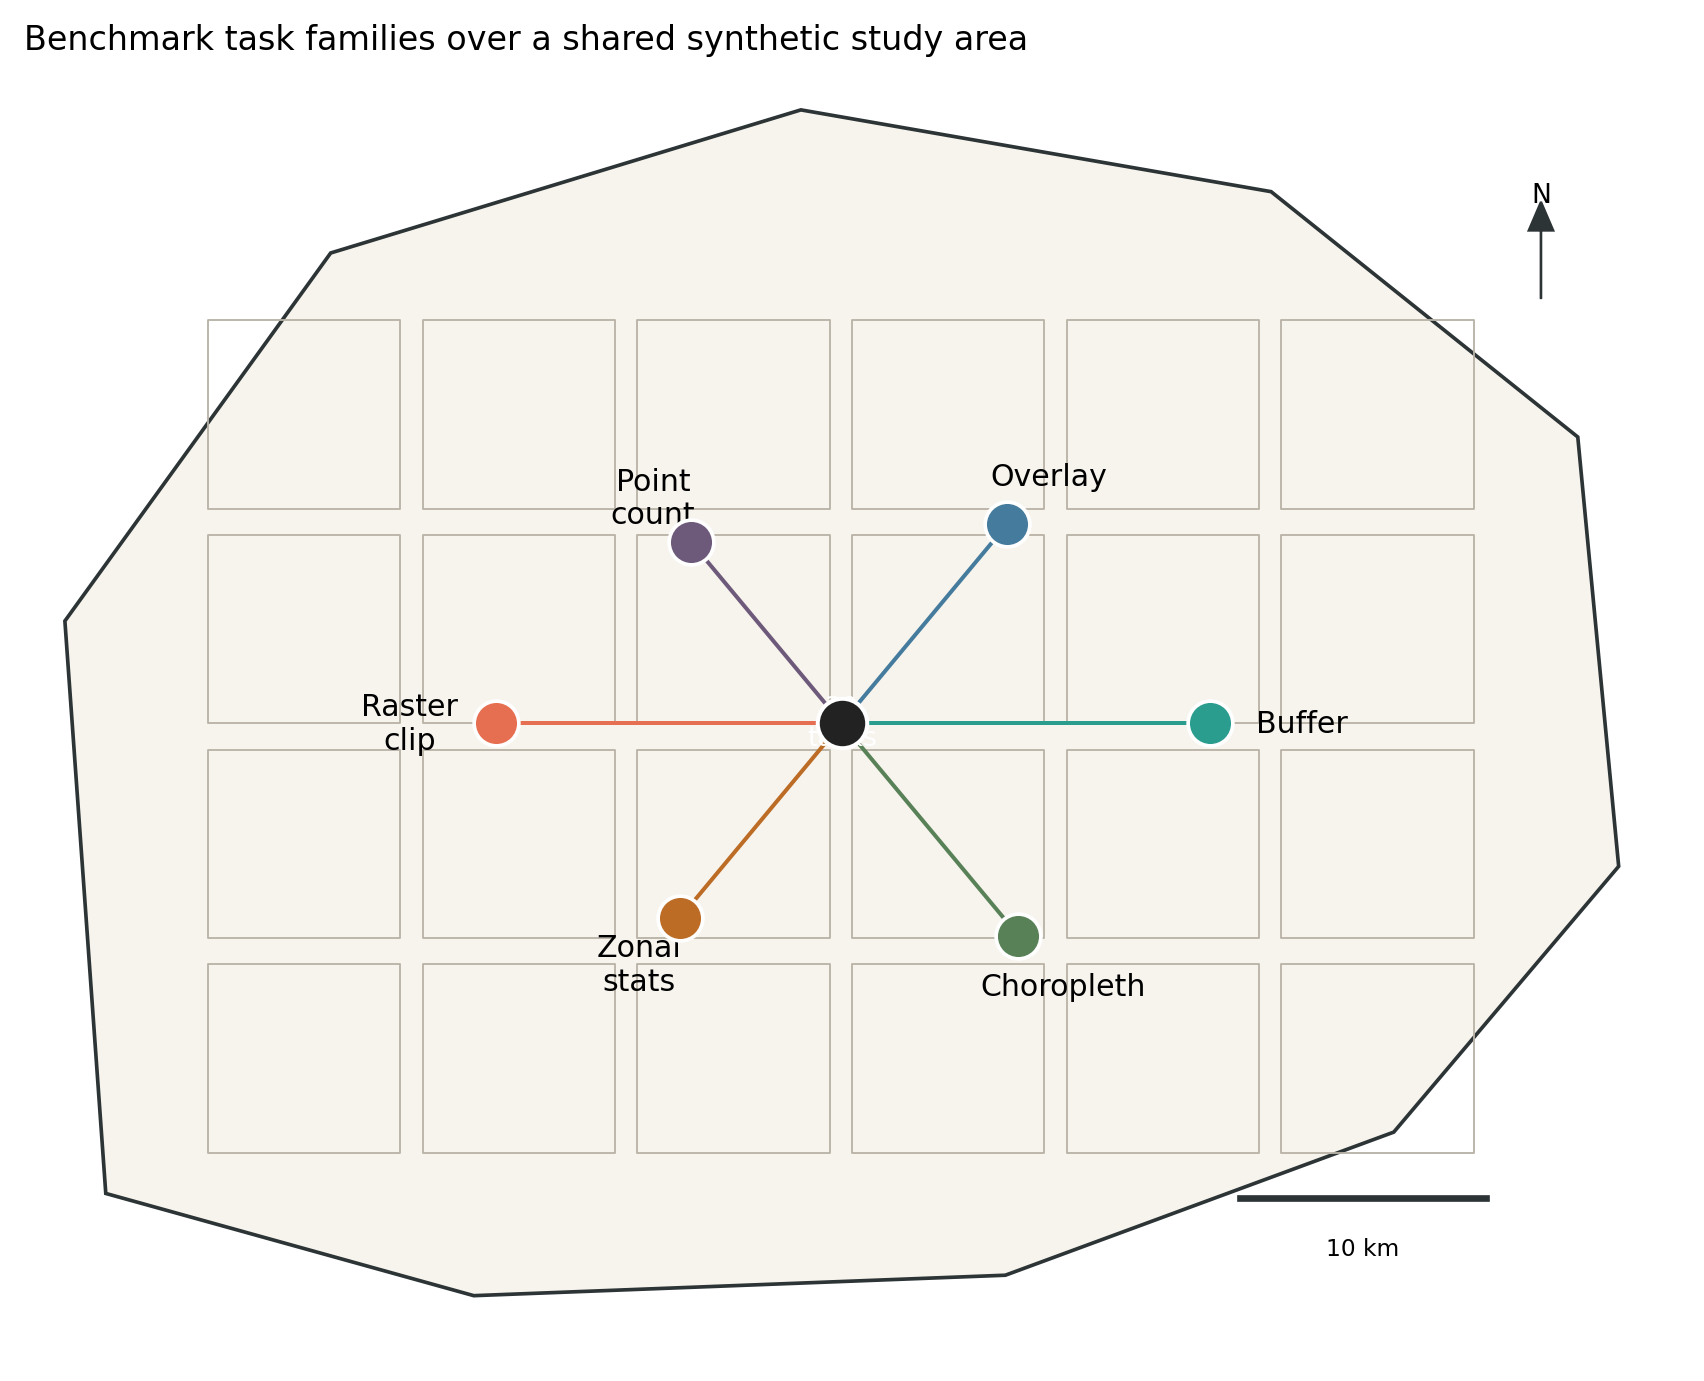
\includegraphics[width=0.78\textwidth]{figures/geo_task_family_coverage.png}
\caption{Geospatial coverage of the six task families in the 30-task suite. Each family probes a different part of the GIS workflow contract: measurement, overlay topology, point-in-polygon aggregation, raster-vector alignment, derived zonal fields, and cartographic export.}
\label{fig:geo-task-family}
\end{figure}

\subsection{Model panel}

The first local model panel contains twelve Ollama models installed on the workstation:

\begin{quote}
qwen2.5-coder:1.5b, qwen2.5-coder:3b, qwen2.5-coder:7b, qwen2.5-coder:14b, qwen2.5-coder:32b, deepseek-coder:6.7b, qwen2.5:3b, qwen3:4b, llama3.2:3b, phi3:mini, mistral:7b, and gemma3:4b.
\end{quote}

The panel deliberately includes more than ten models and mixes coder-specialized models with compact general models. The goal is not only to rank models, but also to test which model families can satisfy a strict JSON workflow-contract protocol. Some models may be useful conversationally while failing the benchmark because they do not produce parseable structured specifications. In this design, that is a legitimate reliability outcome rather than an error to hide.

\subsection{Prompting modes}

Each model is evaluated in three modes:

\begin{itemize}
\item \textit{Basic}: the model receives only the natural-language task, the task identifier, the expected operation type, the required output filename, the required fields, and the JSON schema.
\item \textit{Grounded}: the basic prompt is augmented with a data profile and a list of allowed GIS operations.
\item \textit{GeoGuard}: the grounded prompt is further augmented with validation rules for CRS handling, raster-vector alignment, schema preservation, geometry repair, and map quality.
\end{itemize}

The modes are designed to isolate the effect of grounding and validation. Basic mode tests whether a model can infer a plausible workflow from the user's request. Grounded mode tests whether explicit metadata reduces dataset and field hallucination. GeoGuard mode tests whether validation rules improve the model's planning for CRS, schema, and cartographic output requirements. Figure~\ref{fig:geo-validation-contract} visualizes the intended difference between these modes: the benchmark expects the model to move from a plausible but underspecified map operation toward a validated spatial workflow contract.

\begin{figure}[htbp]
\centering
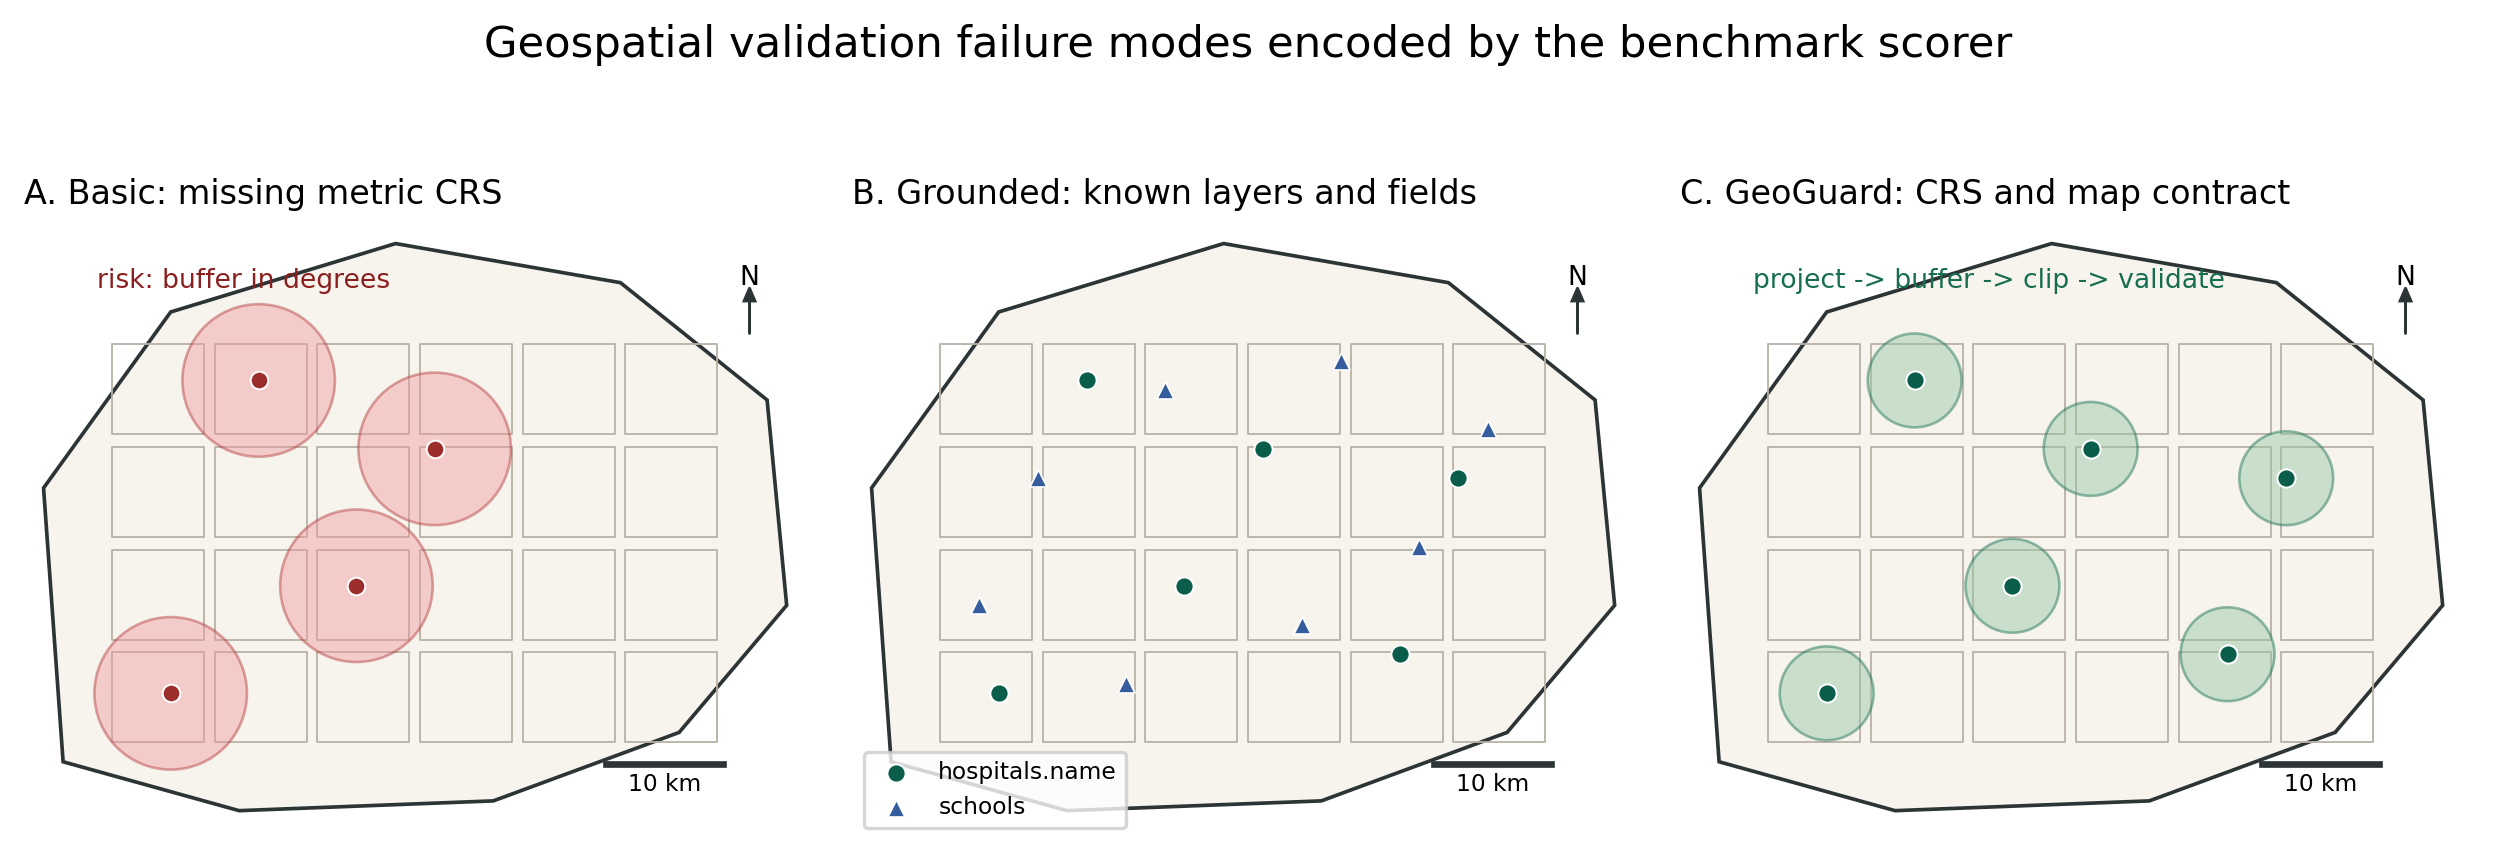
\includegraphics[width=0.98\textwidth]{figures/geo_validation_contract_examples.png}
\caption{Geospatial validation examples encoded by the benchmark scorer. Basic task-only prompting often leaves metric buffering, field provenance, and output map contracts implicit. Grounded prompting exposes known layers and fields, while GeoGuard adds checks for projection, clipping, schema preservation, and cartographic completeness before execution.}
\label{fig:geo-validation-contract}
\end{figure}

\subsection{Workflow schema}

Every response is required to be a single JSON object with the following top-level keys: task identifier, operation, inputs, parameters, output, validation, and rationale. The output object must include a filename, output type, and required fields. The validation object may include CRS, schema, geometry, raster, and map-quality checks. The schema is intentionally simple enough for small local models, but strict enough to reveal malformed responses and implicit assumptions.

Figure~\ref{fig:geo-contract-anatomy} shows how this schema maps onto a GIS artifact. A correct contract links input layers, operation type, validation checks, output schema, and output artifact; omitting any one of these links can leave a downstream executor with an ambiguous or unsafe spatial plan.

\begin{figure}[htbp]
\centering
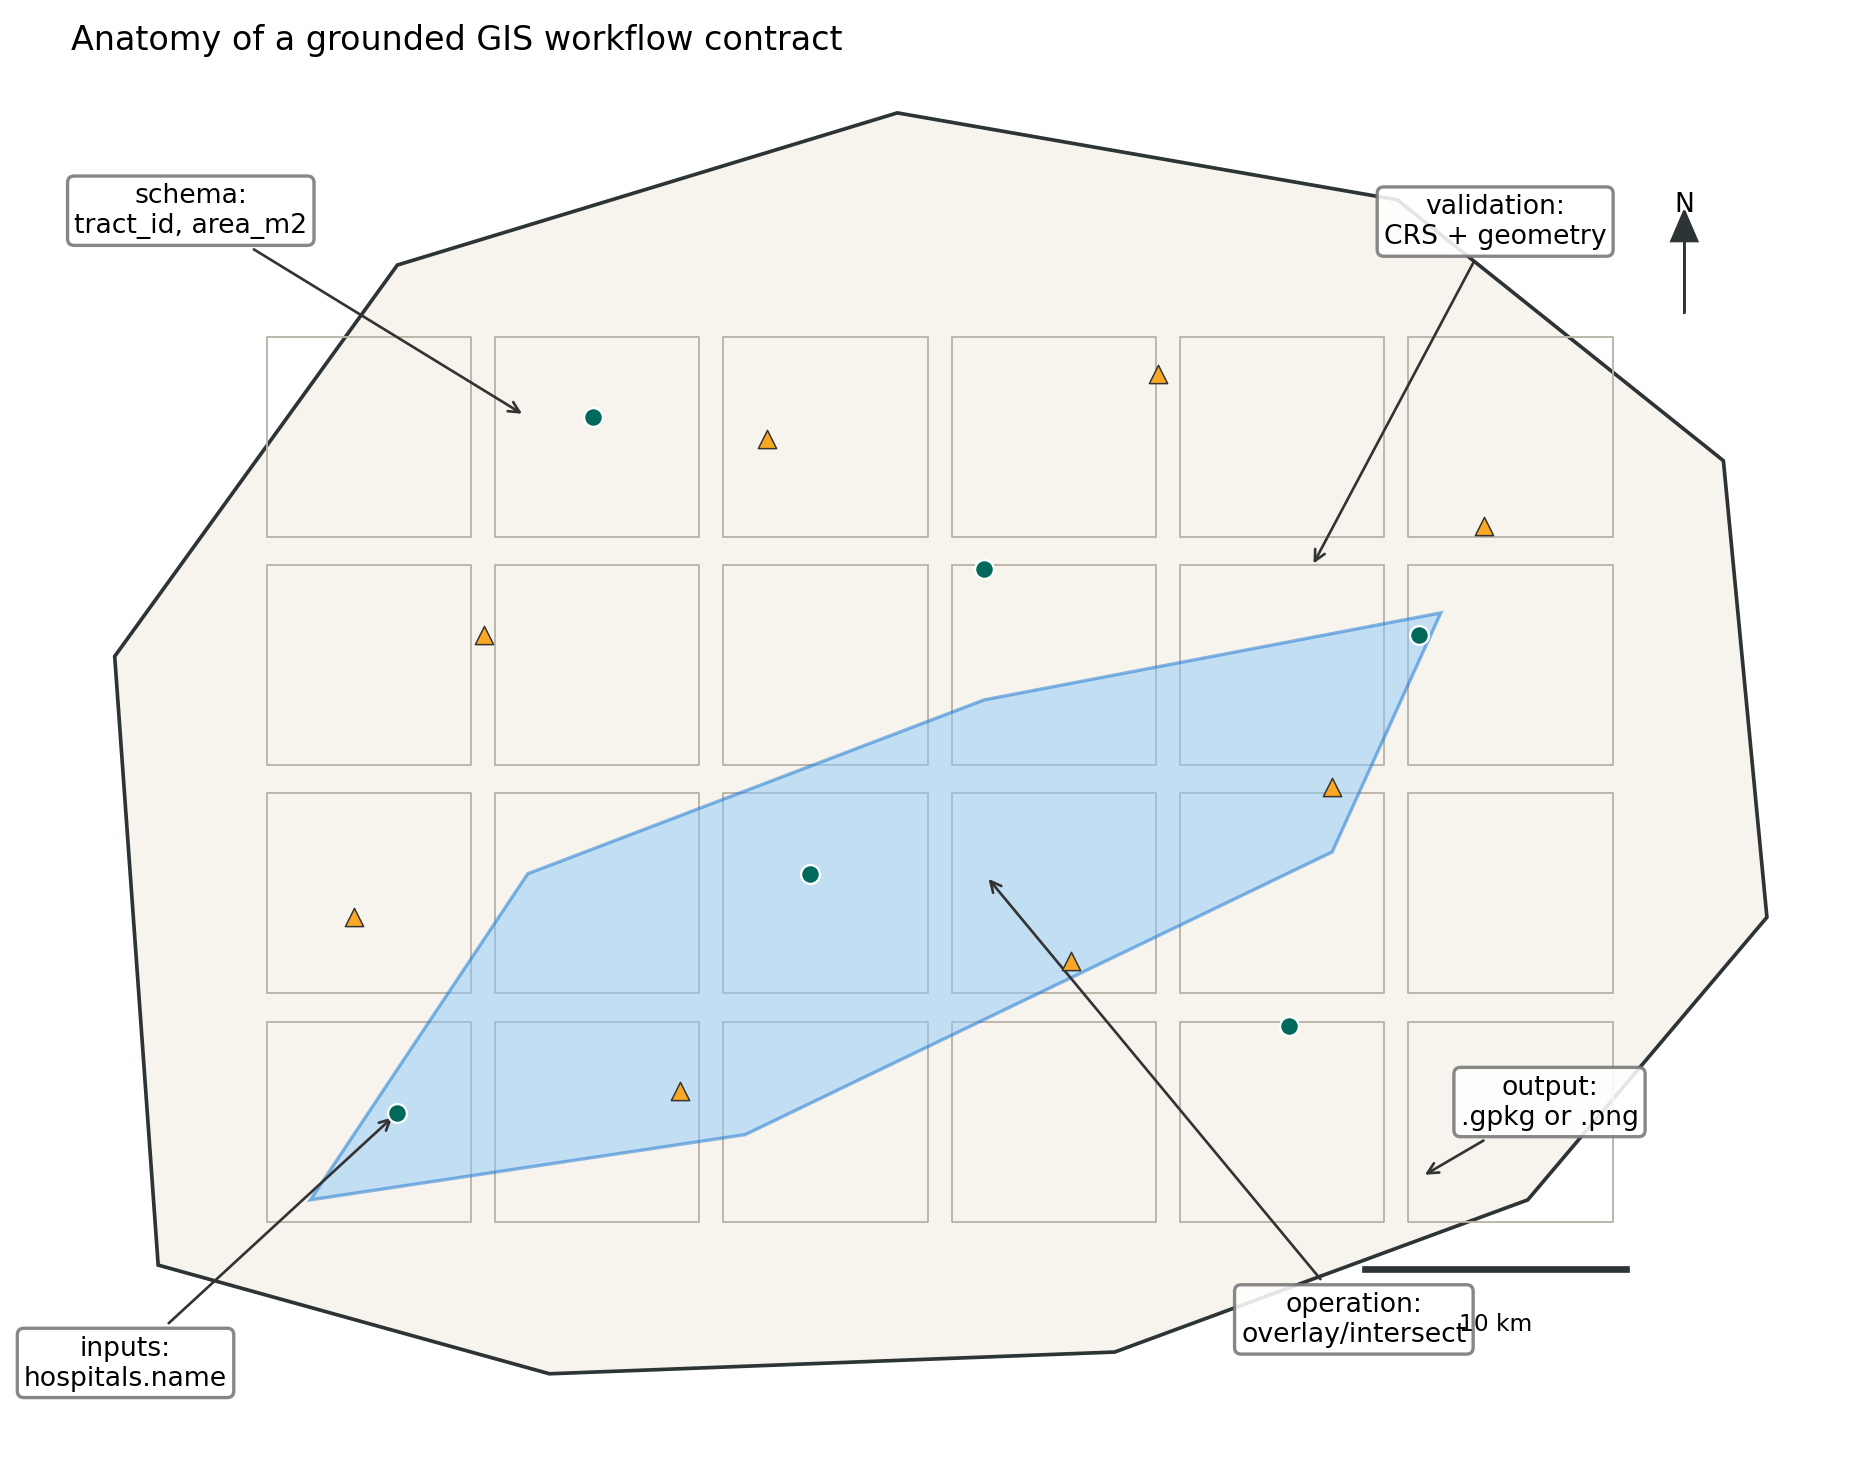
\includegraphics[width=0.82\textwidth]{figures/geo_workflow_contract_anatomy.png}
\caption{Anatomy of a grounded GIS workflow contract. A reliable specification must connect map layers, spatial operation, CRS and geometry validation, output schema, and artifact filename before a deterministic executor or renderer is allowed to run.}
\label{fig:geo-contract-anatomy}
\end{figure}

\subsection{Metrics}

The scorer computes ten plan-level metrics:

\begin{itemize}
\item JSON validity: whether the response is parseable as a JSON object.
\item Tool validity: whether the operation matches the expected task type and belongs to the allowed operation set.
\item Data validity: whether all referenced layers are known layers.
\item Field validity: whether referenced or required fields exist or are created by the operation.
\item CRS plan: whether the plan includes an appropriate CRS strategy.
\item Schema plan: whether required output fields are declared.
\item Map plan: whether map-export tasks include title, legend, classification, color ramp, and source-note requirements.
\item Output name: whether the output filename matches the task.
\item Plan hallucination risk: an unweighted error fraction across tool, data, field, CRS, and filename checks.
\item Plan reliability score: a mean reliability summary across parseability, tool, data, field, CRS, schema, map, output, and inverse weighted hallucination risk.
\end{itemize}

The metrics are not intended as a final theory of GIS correctness. They are a reproducible first layer for comparing model behavior under explicit workflow contracts. Later phases can add execution-level and artifact-level metrics once valid specifications are passed to deterministic executors.

\section{Full Experiment Results}

\subsection{Experimental scope}

The full experiment evaluates twelve local Ollama models over all 30 workflow tasks and three prompting modes. This yields 1080 attempted workflow specifications. Each model-mode pair contributes 30 task rows, and each mode contributes 360 task rows. The panel includes five qwen2.5-coder sizes, one DeepSeek coder model, and six compact or general local models. All models are evaluated under the same prompt protocol and JSON extraction rule; no model-specific prompt repair is applied.

All outputs are generated through the local Ollama HTTP API with deterministic temperature settings. Raw responses, parsed JSON specifications, generation manifests, task-level scores, and aggregate model summaries are written into the experiment track. The full summaries are mirrored into the manuscript table directory so that the manuscript can be rebuilt from recorded evidence rather than from manual notes.

\subsection{Aggregate mode effects}

Table~\ref{tab:mode-summary} and Figure~\ref{fig:mode-profile} summarize the full run by prompting mode. The dominant effect is the difference between task-only planning and metadata-grounded planning. In basic mode, mean data validity is only 0.053 because models frequently invent layer names, use generic filenames, or describe inputs informally. Grounded mode raises data validity to 0.761, increases JSON validity from 0.744 to 0.847, lowers weighted hallucination risk from 0.522 to 0.277, and raises plan reliability score from 0.547 to 0.751. The table gives the exact aggregate values, while the figure makes the mode-level profile easier to compare across metrics.

\begin{table}[htbp]
\centering
\caption{Aggregate full-run performance by prompting mode across twelve local Ollama models and 30 workflow tasks.}
\label{tab:mode-summary}
\small
\setlength{\tabcolsep}{5pt}
\begin{tabular}{lrrrrrrr}
\toprule
Mode & JSON valid & Data valid & Field valid & CRS plan & Map plan & WPHR & PRS \\
\midrule
Basic & 0.744 & 0.053 & 0.309 & 0.569 & 0.662 & 0.522 & 0.547 \\
Grounded & 0.847 & 0.761 & 0.562 & 0.674 & 0.824 & 0.277 & 0.751 \\
GeoGuard & 0.839 & 0.769 & 0.612 & 0.774 & 0.817 & 0.244 & 0.774 \\
\bottomrule
\end{tabular}
\end{table}

Table~\ref{tab:mode-summary} shows that grounding is the main discontinuity in the experiment. The basic-to-grounded jump in data validity is far larger than the grounded-to-GeoGuard change, which indicates that most dataset hallucination is caused by missing data context rather than by weak reasoning alone. GeoGuard's value is narrower but still important: it improves CRS planning and field validity while slightly lowering map-plan score, suggesting that validation-heavy prompts help spatial correctness more than cartographic design completeness. This pattern supports a two-layer prompt design: provide metadata first, then add validation rules for operations where CRS, schema, or raster-vector alignment can change the geographic meaning of the result.

\begin{figure}[htbp]
\centering
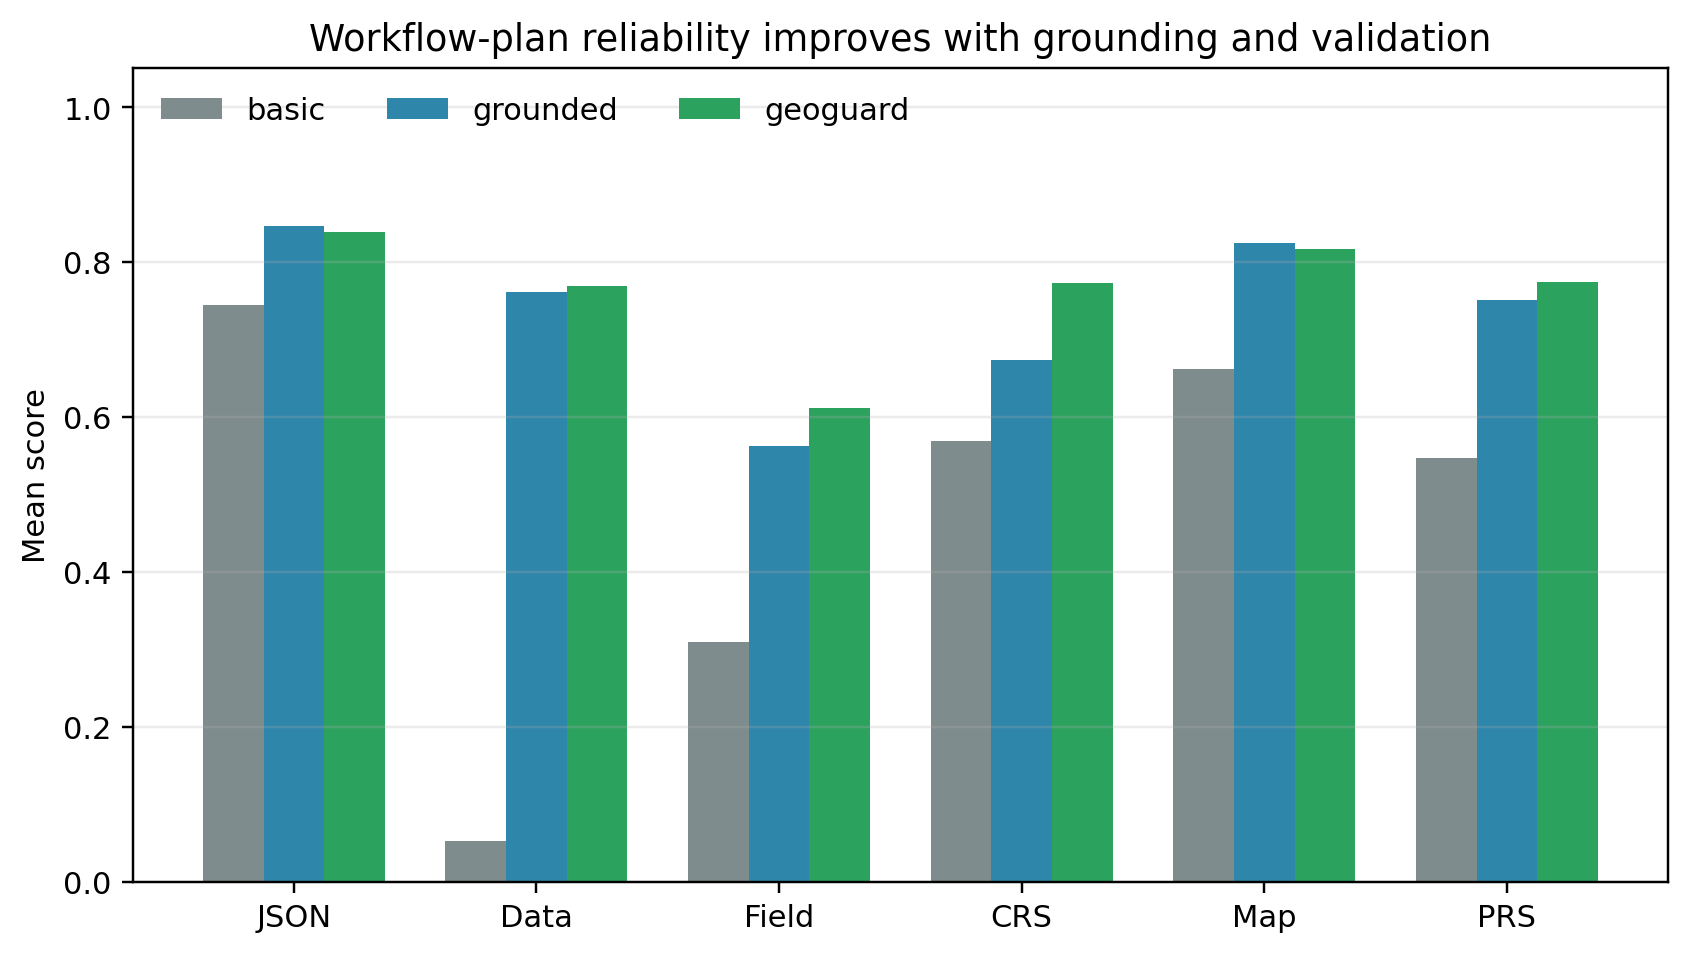
\includegraphics[width=0.92\textwidth]{figures/full_mode_metric_profile.png}
\caption{Mean metric profile by prompting mode across 1080 attempted specifications. Metadata grounding primarily improves data and field validity, while GeoGuard-style validation produces the strongest CRS-planning gains.}
\label{fig:mode-profile}
\end{figure}

The GeoGuard condition produces the strongest CRS-planning effect. Grounded mode tells models what data and tools exist, but it does not always force them to reason consistently about metric buffers, raster masks, or projected area calculations. Adding validation rules raises mean CRS planning from 0.674 in grounded mode to 0.774 in GeoGuard mode and reduces weighted hallucination risk from 0.277 to 0.244. The overall plan reliability increase from grounded to GeoGuard is smaller than the basic-to-grounded jump because some compact models remain unable to satisfy the strict JSON protocol and because map-export tasks expose field and cartographic-plan weaknesses that validation rules do not fully resolve.

\subsection{Failure taxonomy}

Table~\ref{tab:failure-summary} and Figure~\ref{fig:failure-counts} show failure counts by mode. The contrast is starkest for data-invalid failures: basic mode produces 249 data-invalid rows out of 360, while grounded and GeoGuard modes produce only 31 and 25 respectively. This confirms that explicit data profiles are the main intervention against dataset hallucination. Field weakness remains more persistent: basic, grounded, and GeoGuard modes produce 168, 155, and 140 field-weak rows respectively. This indicates that knowing which layers exist does not automatically solve derived-field planning, aggregation fields, or output schema preservation. The table is used for exact counts; the figure emphasizes the relative collapse of data-invalid failures after grounding.

\begin{table}[htbp]
\centering
\caption{Failure counts by prompting mode. Counts are out of 360 task rows per mode.}
\label{tab:failure-summary}
\small
\setlength{\tabcolsep}{4pt}
\begin{tabular}{lrrrrrrrr}
\toprule
Mode & JSON & Tool & Data & Field & CRS & Schema & Map & Output \\
\midrule
Basic & 92 & 2 & 249 & 168 & 83 & 36 & 46 & 9 \\
Grounded & 55 & 8 & 31 & 155 & 89 & 45 & 10 & 19 \\
GeoGuard & 58 & 7 & 25 & 140 & 39 & 33 & 9 & 12 \\
\bottomrule
\end{tabular}
\end{table}

Table~\ref{tab:failure-summary} makes the same result visible as concrete error counts. Basic mode produces 249 data-invalid cases, which means that roughly two thirds of task rows reference unavailable or unsupported data. Grounded and GeoGuard modes reduce this failure class to 31 and 25, respectively, but field-weak cases remain high in all modes. This residual field problem is analytically important: it means that metadata grounding solves ``what layers exist'' better than it solves ``what attributes are preserved, generated, or aggregated.'' The table therefore motivates the later discussion of schema-transition contracts as a missing layer in LLM-GIS workflows.

\begin{figure}[htbp]
\centering
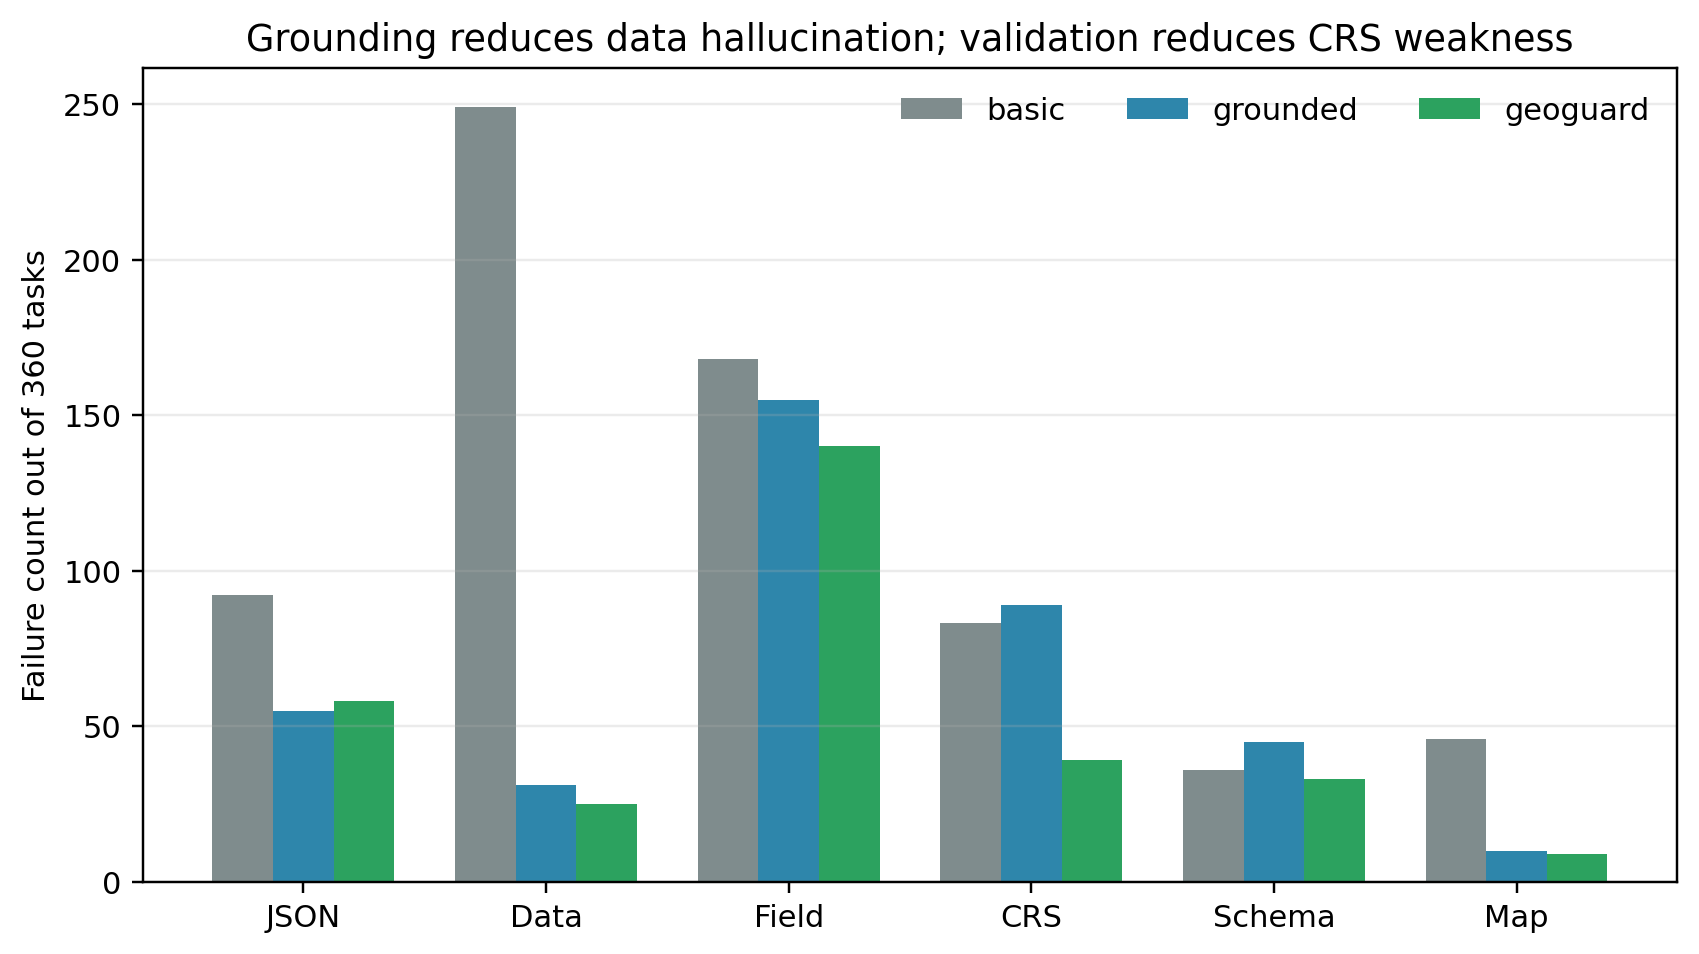
\includegraphics[width=0.92\textwidth]{figures/full_failure_counts_by_mode.png}
\caption{Failure counts across the full 30-task panel. Grounding sharply reduces data hallucination, while GeoGuard-style validation reduces CRS-weak planning. Field weakness remains the most persistent residual failure.}
\label{fig:failure-counts}
\end{figure}

The failure taxonomy also clarifies the distinct roles of grounding and validation. Grounding reduces data-invalid rows because the model no longer needs to guess whether \texttt{hospital\_points}, \texttt{flood\_zones}, \texttt{census\_tracts}, \texttt{temperature\_raster}, or \texttt{zonal\_input\_for\_map} exist. GeoGuard reduces CRS-weak rows because it repeatedly states that metric buffers, area calculations, overlay operations, and raster masks require CRS alignment or projected coordinates. Neither intervention fully solves field weakness. The model must still know that \texttt{school\_count}, \texttt{hospital\_count}, \texttt{flood\_area\_m2}, \texttt{temp\_mean}, and multivariate risk fields are either existing attributes or derived outputs created by a prior operation. Figure~\ref{fig:geo-failure-cases} grounds these abstract failure categories in map examples, showing why a format-valid workflow can still be geospatially unsafe.

\begin{figure}[htbp]
\centering
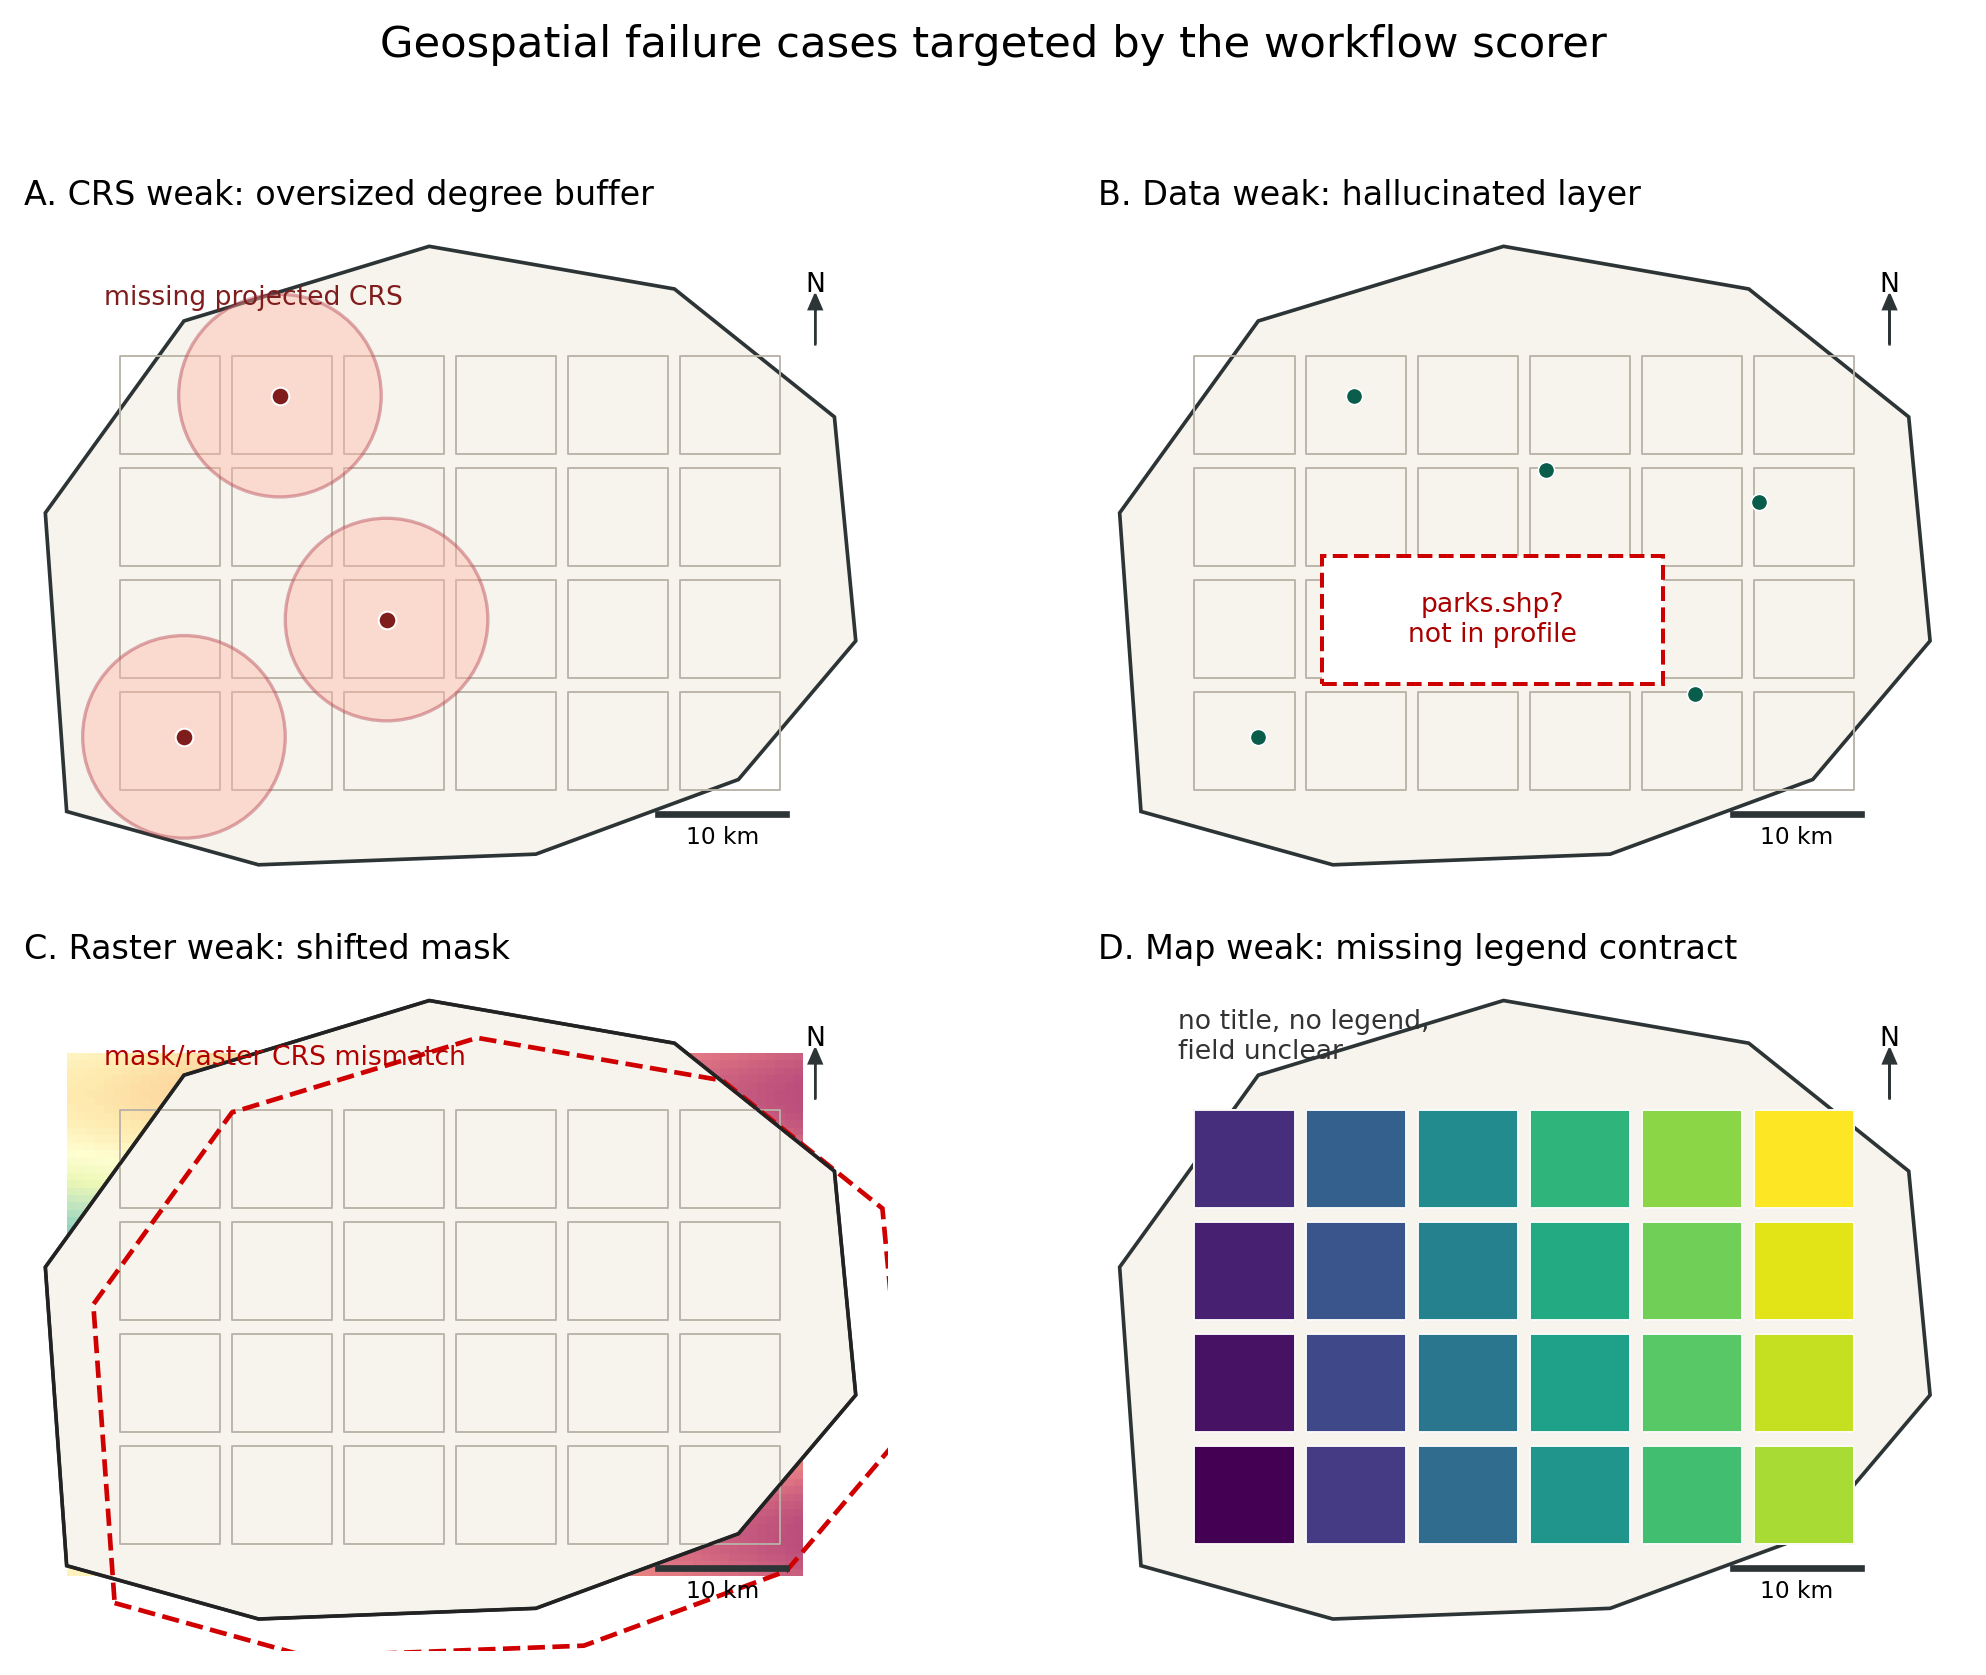
\includegraphics[width=0.96\textwidth]{figures/geo_failure_case_maps.png}
\caption{Representative geospatial failure cases targeted by the scorer. The benchmark treats missing projected CRS, hallucinated layers, shifted raster masks, and incomplete map contracts as distinct reliability failures rather than generic text-generation errors.}
\label{fig:geo-failure-cases}
\end{figure}

\subsection{Model-level behavior}

Table~\ref{tab:model-summary} and Figure~\ref{fig:model-heatmap} report model-level behavior. The strongest GeoGuard PRS values are achieved by qwen2.5-coder:3b (0.947), gemma3:4b (0.945), qwen2.5-coder:14b (0.938), qwen2.5-coder:7b (0.934), qwen2.5-coder:32b (0.934), deepseek-coder:6.7b (0.931), and qwen2.5-coder:1.5b (0.919). This result is important because it does not simply rank the largest model first. Small coder models and a compact general model can emit strong workflow specifications under a structured protocol, while qwen3:4b fails the strict JSON-contract protocol across the full panel. The table provides rankable numeric values, and the heatmap makes the mode sensitivity of each model visible at a glance.

\begin{table}[htbp]
\centering
\caption{Plan reliability score by model and mode in the full 30-task run.}
\label{tab:model-summary}
\small
\setlength{\tabcolsep}{4pt}
\begin{tabular}{lrrr}
\toprule
Model & Basic PRS & Grounded PRS & GeoGuard PRS \\
\midrule
deepseek-coder:6.7b & 0.610 & 0.902 & 0.931 \\
gemma3:4b & 0.773 & 0.911 & 0.945 \\
llama3.2:3b & 0.594 & 0.888 & 0.821 \\
mistral:7b & 0.539 & 0.765 & 0.823 \\
phi3:mini & 0.129 & 0.170 & 0.269 \\
qwen2.5-coder:1.5b & 0.551 & 0.902 & 0.919 \\
qwen2.5-coder:3b & 0.685 & 0.919 & 0.947 \\
qwen2.5-coder:7b & 0.698 & 0.880 & 0.934 \\
qwen2.5-coder:14b & 0.722 & 0.916 & 0.938 \\
qwen2.5-coder:32b & 0.681 & 0.915 & 0.934 \\
qwen2.5:3b & 0.579 & 0.841 & 0.823 \\
qwen3:4b & 0.000 & 0.000 & 0.000 \\
\bottomrule
\end{tabular}
\end{table}

Table~\ref{tab:model-summary} separates model compliance from model scale. The strongest GeoGuard results come from qwen2.5-coder:3b and gemma3:4b, while the larger qwen2.5-coder:32b is strong but not dominant. This suggests that the benchmark rewards structured-output discipline and geospatial contract following rather than parameter count alone. The table also shows two different failure regimes: qwen3:4b has a near-total contract failure under the prompt, whereas phi3:mini improves slightly but remains weak. These rows should not be read simply as ``bad GIS reasoning''; they indicate that some local models need a different structured-output interface before their geospatial reasoning can be evaluated fairly.

\begin{figure}[htbp]
\centering
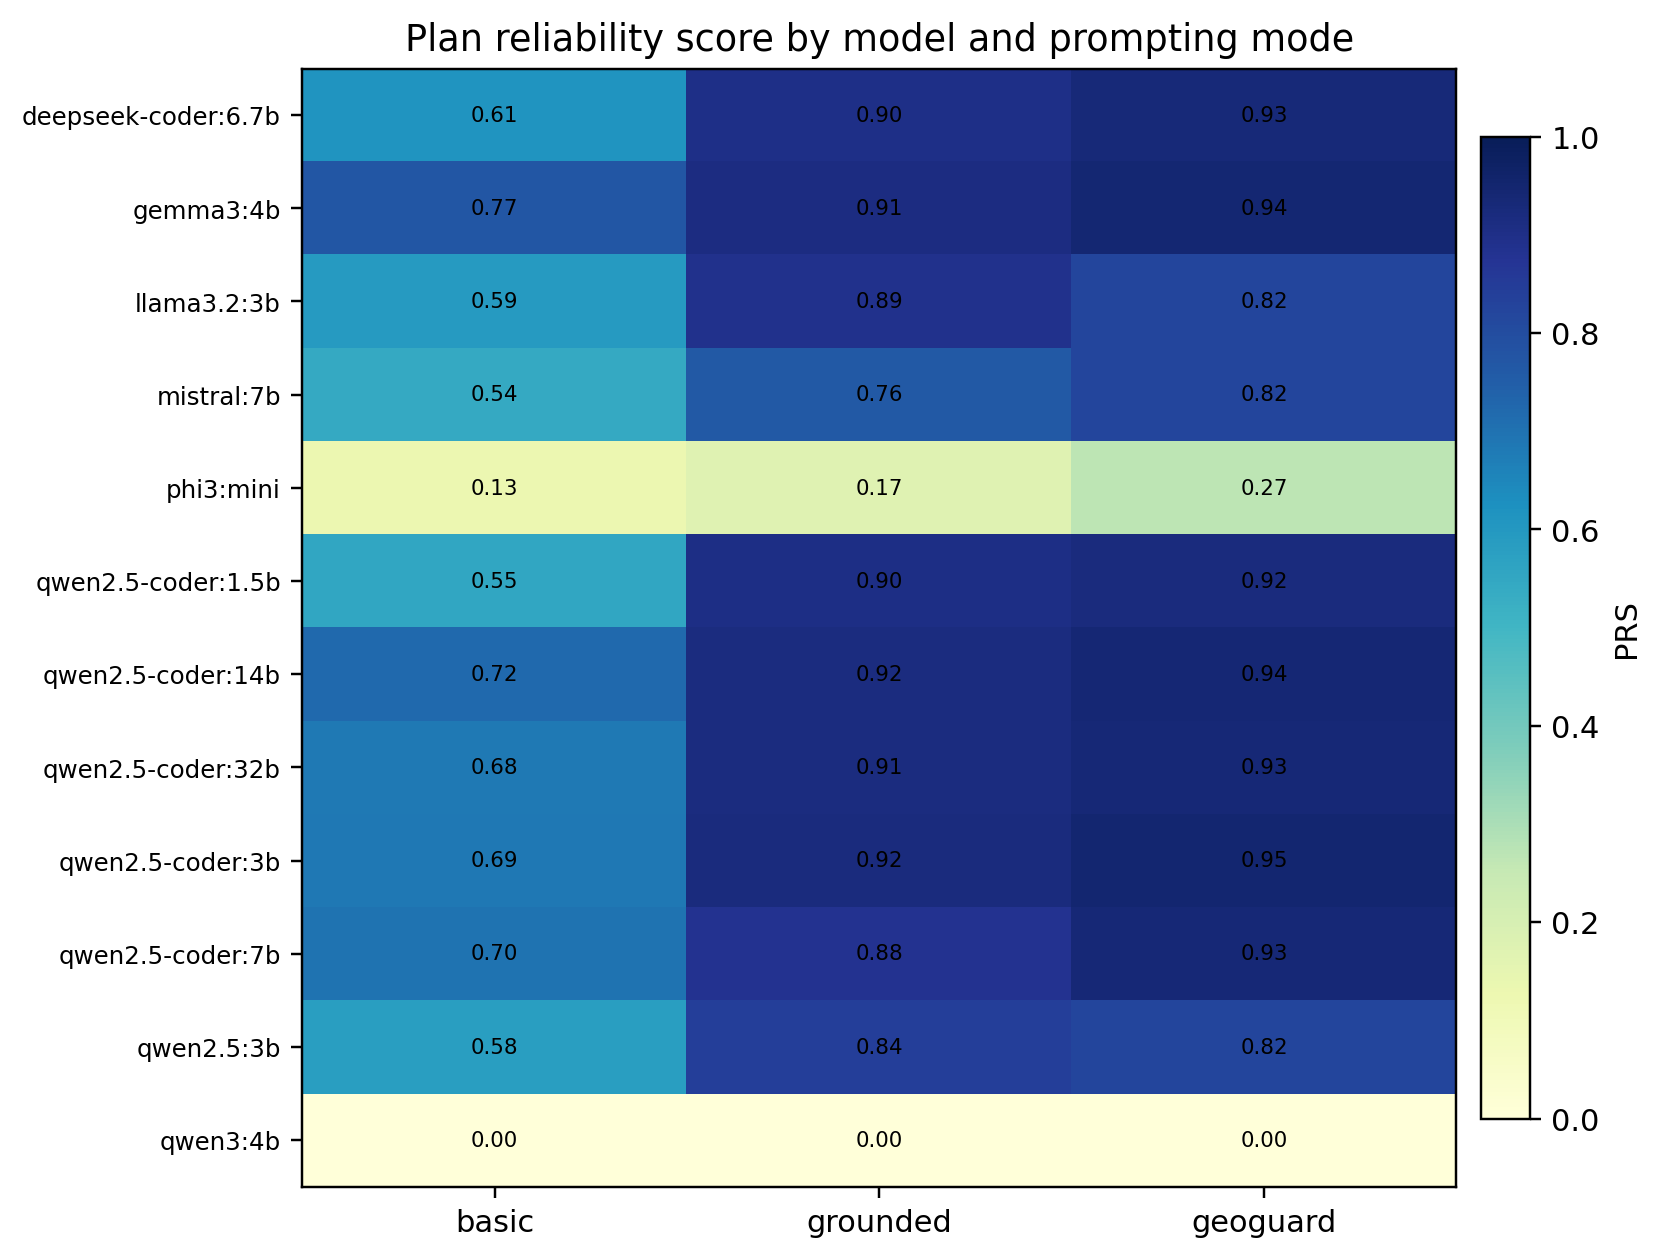
\includegraphics[width=0.78\textwidth]{figures/full_model_prs_heatmap.png}
\caption{Plan reliability score by model and prompting mode. The full panel shows that local structured workflow planning is not a simple function of model size: qwen2.5-coder:3b and gemma3:4b are among the strongest GeoGuard performers, while qwen3:4b fails the strict contract.}
\label{fig:model-heatmap}
\end{figure}

The model-level results separate three capabilities that are often collapsed in LLM-GIS discussion. First, a model must obey the output contract. Qwen3:4b and phi3:mini show that some local models are weak JSON-specification emitters under a uniform prompt even if they may be useful in conversational settings. Second, a model must ground itself in the known data profile. Basic-mode data validity is low for almost every model, including high-scoring basic performers such as gemma3:4b, because task-only prompts leave layer names underspecified. Third, a model must reason about geospatial validity. GeoGuard improves CRS planning for most contract-compliant models, but field validity remains a harder problem because derived schemas require more than recognizing input layers.

\subsection{Task-family effects}

Figure~\ref{fig:category-prs} and Table~\ref{tab:category-summary} show that task families are not equally difficult. Basic-mode buffer tasks are the weakest family, with PRS 0.399, because the models often omit metric buffering and known layer references. GeoGuard lifts buffer PRS to 0.782. Raster clipping is the strongest family under GeoGuard, reaching PRS 0.845, because the validation rules directly match the required raster-mask CRS alignment. Point-count joins also benefit strongly, rising from 0.577 in basic mode to 0.820 in GeoGuard mode. The figure highlights family-level trends, while the table records the exact PRS values used in the comparison.

\begin{figure}[htbp]
\centering
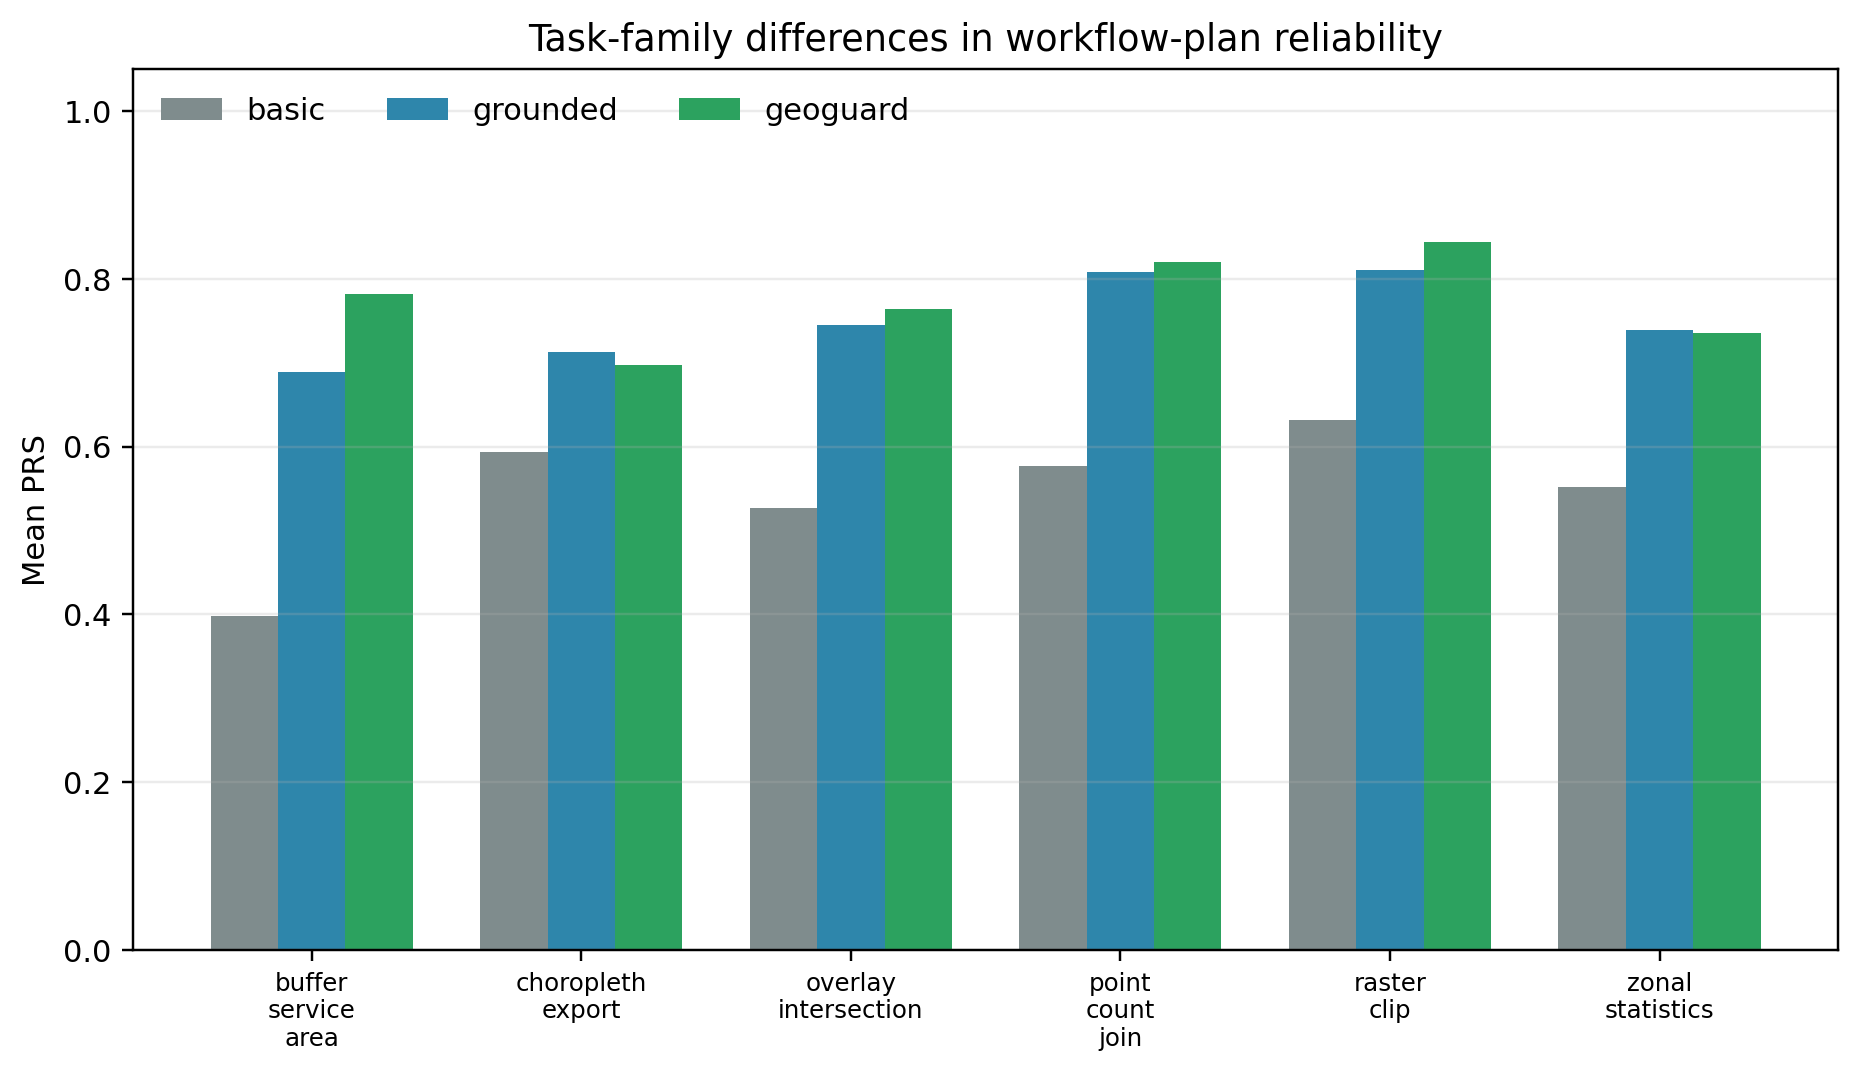
\includegraphics[width=0.95\textwidth]{figures/full_category_prs_by_mode.png}
\caption{Task-family plan reliability scores by prompting mode. Grounding and validation improve all task families, but the strongest gains differ: buffer and point-count tasks benefit sharply from GeoGuard rules, while choropleth export remains limited by field and map-plan weaknesses.}
\label{fig:category-prs}
\end{figure}

\begin{table}[htbp]
\centering
\caption{Plan reliability score by task family and prompting mode. Each cell summarizes 60 task rows.}
\label{tab:category-summary}
\small
\setlength{\tabcolsep}{4pt}
\begin{tabular}{lrrr}
\toprule
Task family & Basic PRS & Grounded PRS & GeoGuard PRS \\
\midrule
Buffer service area & 0.399 & 0.689 & 0.782 \\
Choropleth export & 0.594 & 0.712 & 0.697 \\
Overlay intersection & 0.527 & 0.746 & 0.764 \\
Point-count join & 0.577 & 0.808 & 0.820 \\
Raster clip & 0.632 & 0.811 & 0.845 \\
Zonal statistics & 0.552 & 0.739 & 0.735 \\
\bottomrule
\end{tabular}
\end{table}

Table~\ref{tab:category-summary} shows that task family is a major source of variance. Raster clip is the strongest GeoGuard family because its central requirement, raster-mask CRS alignment, is directly named by the validation rules. Buffer tasks show the largest relative improvement because metric CRS guidance corrects a common basic-mode weakness. Choropleth export is the exception: GeoGuard does not outperform grounded prompting because map export depends on thematic-field choice and cartographic design, not only on geospatial validity checks. This family-level pattern argues that GIS copilots need separate validation modules for spatial analysis and map communication.

Choropleth export behaves differently. Grounded mode slightly outperforms GeoGuard in PRS, 0.712 versus 0.697, because GeoGuard introduces more validation context without fully solving the harder question of which derived field a map should use. In this family, map plan improves relative to basic mode, but field validity remains weak. This result is cartographically important. A workflow can name the correct data layer and still fail to state a defensible thematic field, classification scheme, or legend contract. Map production therefore needs a cartographic design contract in addition to GIS validity rules. Figure~\ref{fig:geo-cartographic-variants} illustrates this distinction: the same tract geometry can be a weak map, a grounded thematic map, or a publication-ready export depending on whether the workflow contract includes cartographic elements.

\begin{figure}[htbp]
\centering
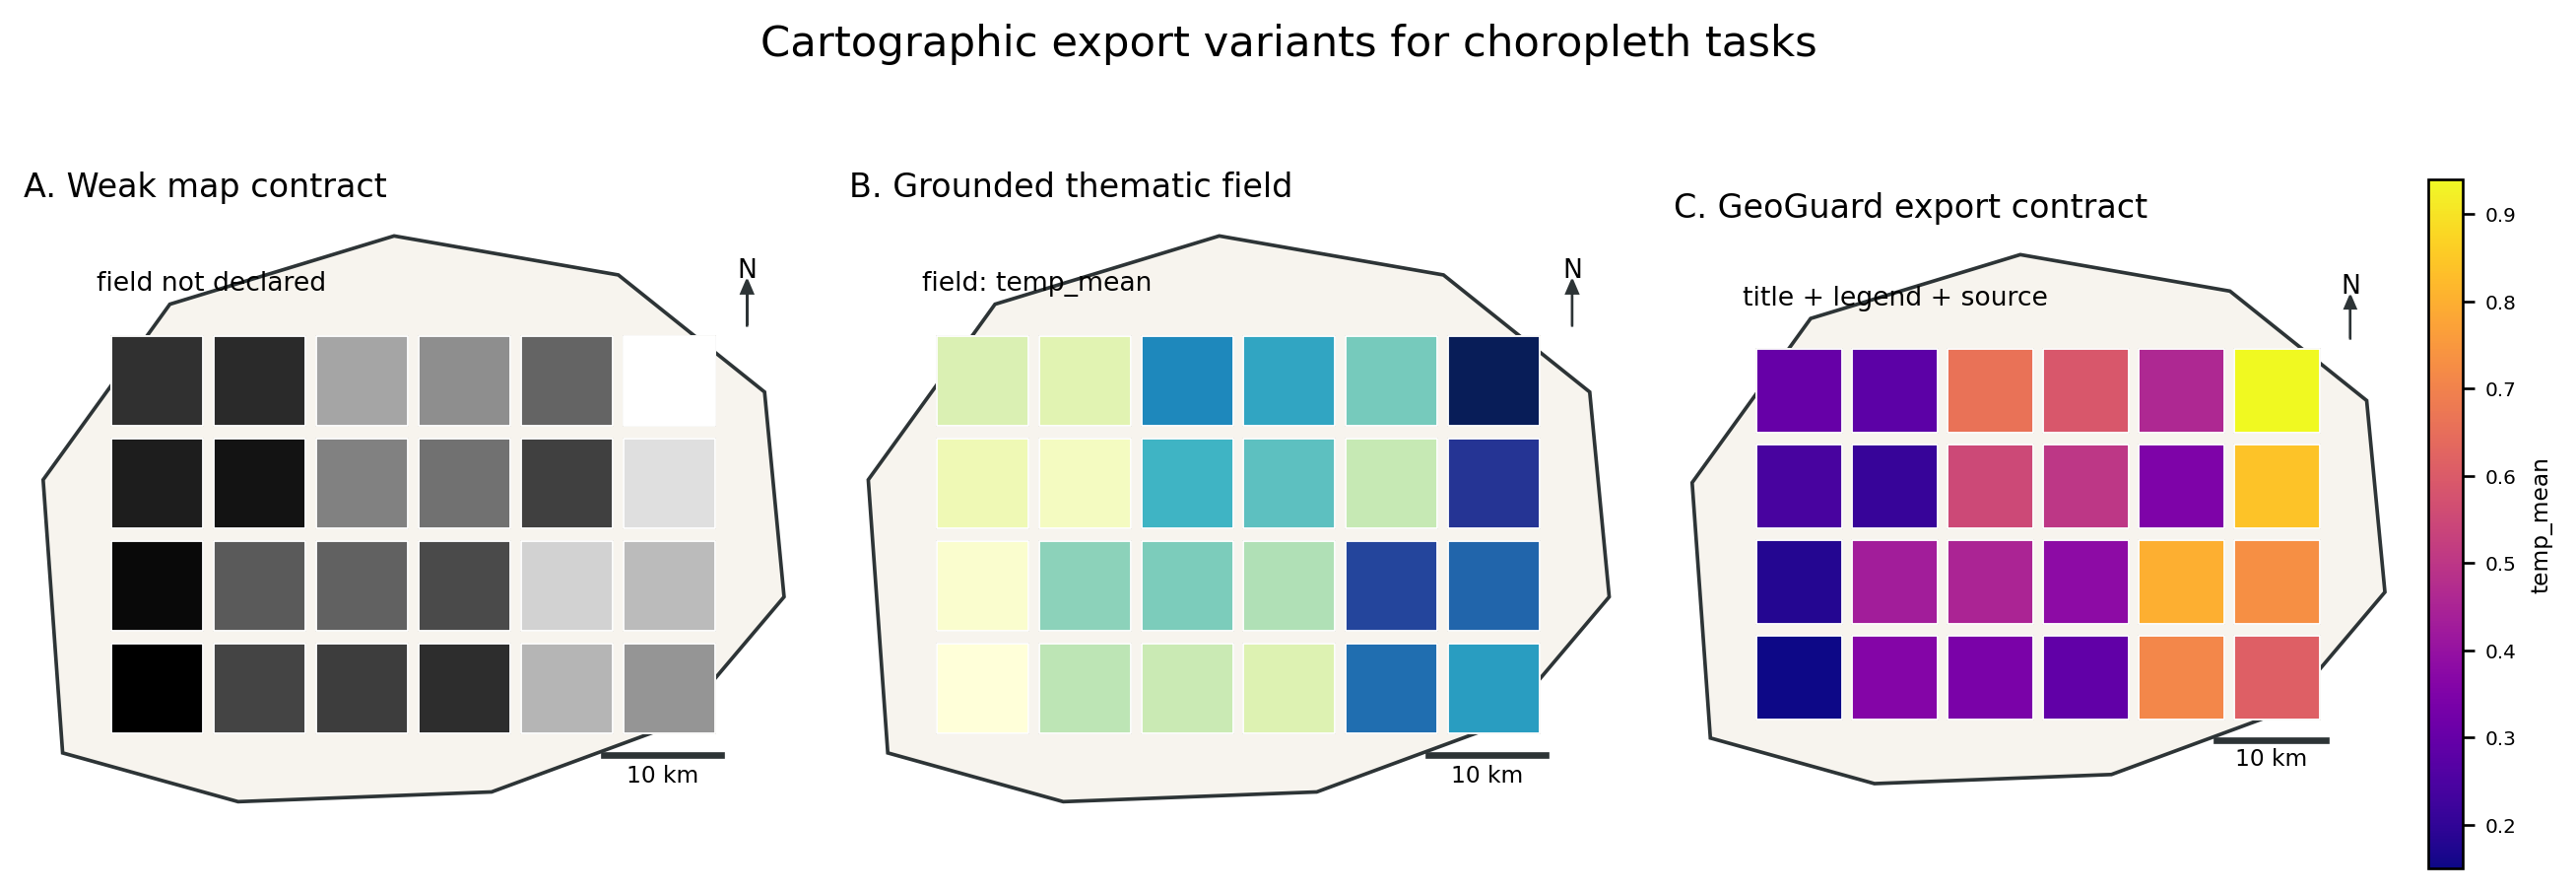
\includegraphics[width=0.98\textwidth]{figures/geo_cartographic_export_variants.png}
\caption{Cartographic export variants for choropleth tasks. The map family requires more than a valid layer reference: the workflow contract must identify a thematic field, classification or color strategy, title, legend, and source-note requirements.}
\label{fig:geo-cartographic-variants}
\end{figure}

\section{Discussion}

\subsection{Why workflow specifications matter}

The full experiment supports the premise that workflow specifications are a useful evaluation layer. They expose geospatial hallucination before code execution, and they allow controlled comparison of grounding strategies. If a model cannot name the correct input layers, preserve required fields, or state a CRS strategy for a buffer, overlay, raster mask, or zonal statistic, downstream code generation is unlikely to be trustworthy. Conversely, a valid specification can be inspected, repaired, or executed by deterministic tooling.

This is not a replacement for code execution or map-quality review. It is a preceding layer. A complete LLM-GIS copilot should still be evaluated for execution success, artifact readability, cartographic design, and user-facing interpretation. The contribution of the present benchmark is to isolate planning reliability so that later failures can be attributed more clearly.

\subsection{Grounding versus validation}

The difference between grounded and GeoGuard modes is instructive. Grounding largely solves dataset hallucination by telling models what layers and operations exist. Validation rules mainly improve CRS planning. This division suggests that GIS-copilot prompts should not treat all context as the same. Data profiles answer the question ``what exists?'' Tool schemas answer ``what can be done?'' Validation rules answer ``what must be true for the operation to be spatially valid?'' A robust copilot architecture should provide all three.

The residual field-validity problem is a different kind of error. It is not enough for the model to know that a layer exists. It must also know when a field is an input attribute, when it is an output attribute created by an operation, and when it is a derived design variable that requires a previous analysis step. This explains why field weakness remains high even after grounding and validation. The benchmark therefore suggests a fourth context layer for future GIS copilots: an explicit schema-transition contract that describes which fields are preserved, generated, aggregated, or consumed by each operation.

\subsection{Task families as diagnostic probes}

The six task families diagnose different parts of the GIS-copilot stack. Buffer tasks stress measurement units and projected CRS selection. Overlay tasks stress multi-layer alignment and output-field preservation. Point-count joins stress spatial predicates and generated count fields. Raster clips stress raster-vector CRS alignment and nodata handling. Zonal statistics stress raster-vector interaction plus derived statistical fields. Choropleth export stresses cartographic communication rather than spatial analysis alone.

This decomposition matters because a single average score can hide very different failure modes. Raster clipping has the highest GeoGuard PRS because the validation rule directly matches the operation's central risk: align the mask to the raster CRS before clipping. Choropleth export remains weaker because the operation is underspecified if the model has to choose a thematic field, classification, color ramp, title, legend, and source note from a derived or ambiguous layer. These cartographic choices are not solved by a generic CRS validator. They require a map-design contract that is closer to cartographic specification than to ordinary GIS preprocessing.

\subsection{Local model implications}

The experiment was intentionally restricted to locally installed Ollama models. This choice matters for reproducibility and cost: all generations can be rerun without cloud APIs, rate limits, or proprietary model access. It also reveals the heterogeneity of local models. Some compact models are not suitable for strict JSON workflow planning under the present prompt. Others, including small coder models, perform strongly across the full 30-task panel when grounded and constrained.

The model rankings should still be read as workflow-contract rankings rather than universal LLM rankings. The benchmark rewards models that emit strict JSON, name known layers, declare required fields, and state validation checks. A model that fails this protocol may still be useful with a different prompting interface or a native structured-output API. Conversely, a high workflow-specification score does not prove that the generated specification will execute successfully or produce a publication-quality map. It shows that the plan is structured enough for the next layer of deterministic execution and artifact validation.

The strongest practical finding is that smaller local models can be competitive when the task is framed as structured planning rather than free-form code generation. Qwen2.5-coder:3b and gemma3:4b are among the strongest GeoGuard performers, and qwen2.5-coder:1.5b remains above 0.91 PRS. This matters for reproducible GIS-assistant research because local inference avoids proprietary APIs, rate limits, and model-version drift. The result does not imply that these models can replace stronger cloud models for open-ended GIS coding. It shows that a constrained workflow-contract interface can make local models useful for a narrower but operationally important planning role.

\section{Limitations and Next Steps}

This draft reports the full planning sweep, but it does not yet include deterministic execution of accepted specifications. The evidence covers twelve models, three modes, and 30 tasks, yielding 1080 attempted specifications. The next experimental layer should convert valid workflow specifications into deterministic executor calls and compare plan-level validity with execution success, artifact validity, and rendered map quality.

The current scorer is rule-based. It checks explicit layer names, field references, CRS signals, schema declarations, map-plan tokens, and output filenames. This is appropriate for a reproducible first pass, but it cannot assess every plausible workflow representation. Future versions should add a deterministic executor for accepted specs, then compare plan-level validity with execution-level success and artifact-level cartographic quality.

The benchmark also uses a single prompt template per mode. Some models, especially qwen3:4b and phi3:mini, may improve with model-specific format controls. This paper deliberately avoids per-model prompt tuning because the goal is a uniform contract. A later robustness analysis can compare uniform prompting with model-specific structured-output prompting.

Finally, the current benchmark uses synthetic but realistic task contracts over a fixed data profile. This is appropriate for isolating planning behavior, but it does not cover the full diversity of GIS practice. Future task sets should include temporal joins, network analysis, raster resampling, uncertainty propagation, scale-dependent cartographic generalization, and interactive web-map export. They should also include adversarial prompts that intentionally mention unavailable layers or ambiguous fields, because real users often phrase GIS requests with incomplete data knowledge.

\section{Supplementary Full-Run Tables}

This section records the main full-run tables inside the manuscript draft so the paper can be read without opening the experiment directory. The complete CSV ledgers remain in the repository and should be treated as the reproducibility source of record. Table~\ref{tab:appendix-model-mode} gives the complete model-by-mode metric profile, and Table~\ref{tab:appendix-failure-family} gives the corresponding family-level failure counts.

\begin{table}[htbp]
\centering
\caption{Full model-by-mode reliability metrics.}
\label{tab:appendix-model-mode}
\small
\setlength{\tabcolsep}{3pt}
\begin{tabular}{llrrrrrr}
\toprule
Model & Mode & JSON & Data & Field & CRS & WPHR & PRS \\
\midrule
deepseek-coder:6.7b & Basic & 0.800 & 0.067 & 0.372 & 0.633 & 0.479 & 0.610 \\
deepseek-coder:6.7b & Grounded & 1.000 & 0.867 & 0.646 & 0.783 & 0.141 & 0.902 \\
deepseek-coder:6.7b & GeoGuard & 1.000 & 0.900 & 0.682 & 0.933 & 0.097 & 0.931 \\
gemma3:4b & Basic & 1.000 & 0.133 & 0.586 & 0.833 & 0.320 & 0.773 \\
gemma3:4b & Grounded & 1.000 & 1.000 & 0.690 & 0.750 & 0.123 & 0.911 \\
gemma3:4b & GeoGuard & 1.000 & 0.967 & 0.817 & 0.867 & 0.077 & 0.945 \\
llama3.2:3b & Basic & 0.867 & 0.067 & 0.178 & 0.567 & 0.524 & 0.594 \\
llama3.2:3b & Grounded & 0.967 & 0.967 & 0.760 & 0.883 & 0.120 & 0.888 \\
llama3.2:3b & GeoGuard & 0.900 & 0.900 & 0.547 & 0.817 & 0.194 & 0.821 \\
mistral:7b & Basic & 0.800 & 0.067 & 0.244 & 0.700 & 0.536 & 0.539 \\
mistral:7b & Grounded & 1.000 & 0.867 & 0.390 & 0.750 & 0.215 & 0.765 \\
mistral:7b & GeoGuard & 0.967 & 0.867 & 0.463 & 0.917 & 0.164 & 0.823 \\
phi3:mini & Basic & 0.200 & 0.000 & 0.067 & 0.200 & 0.903 & 0.129 \\
phi3:mini & Grounded & 0.267 & 0.200 & 0.133 & 0.200 & 0.827 & 0.170 \\
phi3:mini & GeoGuard & 0.300 & 0.300 & 0.180 & 0.300 & 0.713 & 0.269 \\
qwen2.5:3b & Basic & 0.833 & 0.000 & 0.244 & 0.650 & 0.520 & 0.579 \\
qwen2.5:3b & Grounded & 1.000 & 0.633 & 0.564 & 0.817 & 0.222 & 0.841 \\
qwen2.5:3b & GeoGuard & 0.933 & 0.667 & 0.488 & 0.750 & 0.221 & 0.823 \\
qwen2.5-coder:1.5b & Basic & 0.767 & 0.100 & 0.322 & 0.333 & 0.587 & 0.551 \\
qwen2.5-coder:1.5b & Grounded & 1.000 & 0.867 & 0.832 & 0.750 & 0.143 & 0.902 \\
qwen2.5-coder:1.5b & GeoGuard & 1.000 & 0.800 & 0.878 & 0.967 & 0.107 & 0.919 \\
qwen2.5-coder:3b & Basic & 0.900 & 0.067 & 0.378 & 0.733 & 0.404 & 0.685 \\
qwen2.5-coder:3b & Grounded & 1.000 & 0.967 & 0.694 & 0.750 & 0.118 & 0.919 \\
qwen2.5-coder:3b & GeoGuard & 1.000 & 0.967 & 0.788 & 0.867 & 0.076 & 0.947 \\
qwen2.5-coder:7b & Basic & 0.933 & 0.000 & 0.378 & 0.733 & 0.404 & 0.698 \\
qwen2.5-coder:7b & Grounded & 0.967 & 0.867 & 0.836 & 0.783 & 0.150 & 0.880 \\
qwen2.5-coder:7b & GeoGuard & 1.000 & 0.900 & 0.861 & 0.983 & 0.085 & 0.934 \\
qwen2.5-coder:14b & Basic & 0.933 & 0.067 & 0.411 & 0.767 & 0.369 & 0.722 \\
qwen2.5-coder:14b & Grounded & 0.967 & 0.967 & 0.817 & 0.783 & 0.107 & 0.916 \\
qwen2.5-coder:14b & GeoGuard & 0.967 & 0.967 & 0.816 & 0.917 & 0.082 & 0.938 \\
qwen2.5-coder:32b & Basic & 0.900 & 0.067 & 0.354 & 0.683 & 0.419 & 0.681 \\
qwen2.5-coder:32b & Grounded & 1.000 & 0.933 & 0.810 & 0.833 & 0.111 & 0.915 \\
qwen2.5-coder:32b & GeoGuard & 1.000 & 1.000 & 0.842 & 0.967 & 0.078 & 0.934 \\
qwen3:4b & Basic & 0.000 & 0.000 & 0.000 & 0.000 & 1.000 & 0.000 \\
qwen3:4b & Grounded & 0.000 & 0.000 & 0.000 & 0.000 & 1.000 & 0.000 \\
qwen3:4b & GeoGuard & 0.000 & 0.000 & 0.000 & 0.000 & 1.000 & 0.000 \\
\bottomrule
\end{tabular}
\end{table}

Table~\ref{tab:appendix-model-mode} is useful for audit because it preserves secondary metrics that are compressed in the main model summary, including JSON validity, data validity, field validity, CRS planning, and weighted hallucination risk. It shows, for example, that several strong GeoGuard models still differ in field validity even when their aggregate PRS values are close. The table also reveals why PRS alone should not be treated as the only ranking criterion: qwen2.5-coder:7b and qwen2.5-coder:32b have similar GeoGuard PRS values, but they arrive there through different field-validity and CRS-planning profiles. For a deployed GIS copilot, this distinction matters because a workflow that is CRS-safe but field-weak will fail differently from one that preserves schema but omits a projection strategy.

\begin{table}[htbp]
\centering
\caption{Failure counts by task family and prompting mode. Counts are out of 60 rows per family-mode pair.}
\label{tab:appendix-failure-family}
\small
\setlength{\tabcolsep}{3pt}
\begin{tabular}{llrrrrrr}
\toprule
Task family & Mode & JSON & Data & Field & CRS & Map & Output \\
\midrule
Buffer & Basic & 24 & 35 & 32 & 52 & 0 & 5 \\
Buffer & Grounded & 12 & 4 & 17 & 48 & 0 & 7 \\
Buffer & GeoGuard & 11 & 1 & 10 & 19 & 0 & 2 \\
Choropleth & Basic & 14 & 46 & 3 & 0 & 46 & 1 \\
Choropleth & Grounded & 10 & 11 & 11 & 0 & 10 & 2 \\
Choropleth & GeoGuard & 12 & 8 & 14 & 0 & 9 & 4 \\
Overlay & Basic & 13 & 43 & 56 & 25 & 0 & 1 \\
Overlay & Grounded & 6 & 7 & 34 & 31 & 0 & 4 \\
Overlay & GeoGuard & 10 & 4 & 24 & 26 & 0 & 2 \\
Point-count & Basic & 11 & 49 & 50 & 16 & 0 & 1 \\
Point-count & Grounded & 7 & 4 & 34 & 7 & 0 & 3 \\
Point-count & GeoGuard & 6 & 4 & 25 & 6 & 0 & 1 \\
Raster & Basic & 17 & 37 & 0 & 22 & 0 & 0 \\
Raster & Grounded & 10 & 5 & 0 & 10 & 0 & 0 \\
Raster & GeoGuard & 8 & 7 & 0 & 8 & 0 & 0 \\
Zonal & Basic & 13 & 39 & 27 & 20 & 0 & 1 \\
Zonal & Grounded & 10 & 0 & 59 & 0 & 0 & 3 \\
Zonal & GeoGuard & 11 & 1 & 57 & 0 & 0 & 3 \\
\bottomrule
\end{tabular}
\end{table}

Table~\ref{tab:appendix-failure-family} shows which failure categories dominate each task family. Buffer tasks concentrate CRS weaknesses, choropleth tasks concentrate map-plan weaknesses, and zonal tasks concentrate field/schema weaknesses, matching the diagnostic interpretation in the main results. The family-mode breakdown is useful because it prevents an overly broad conclusion such as ``GeoGuard fixes GIS errors.'' It does not. GeoGuard sharply reduces CRS-weak buffer cases, but it leaves many zonal field-weak cases unresolved and only modestly improves choropleth map-plan failures. The table therefore identifies where additional experiment design is needed: schema-transition rules for zonal/aggregation tasks and explicit cartographic contracts for export tasks.

\clearpage
\section{Compact Experimental Ledgers}

The previous tables summarize the full run at model and family levels. The following compact ledgers make the experimental basis explicit without printing every generated row. Table~\ref{tab:task-suite-long} lists the complete 30-task suite, Table~\ref{tab:task-prs-matrix} gives a task-level PRS matrix across modes, Table~\ref{tab:geoguard-model-family-matrix} gives a GeoGuard model-by-family matrix, and Table~\ref{tab:geoguard-hard-cases} lists the lowest-scoring GeoGuard task-model cases after removing malformed JSON responses. The complete CSV ledgers, including all 1080 task-level rows and the full category-by-model-by-mode summaries, remain in the repository and are the reproducibility source of record.

\begin{longtable}{p{0.08\linewidth}p{0.18\linewidth}p{0.28\linewidth}p{0.34\linewidth}}
\caption{Complete 30-task workflow-specification suite.}\label{tab:task-suite-long}\\
\toprule
Task & Family & Required fields & Output artifact \\
\midrule
\endfirsthead
\toprule
Task & Family & Required fields & Output artifact \\
\midrule
\endhead
T001 & Buffer & name & T001\_buffer\_hospitals.gpkg \\
T002 & Buffer & name & T002\_buffer\_hospitals\_2500m.gpkg \\
T003 & Buffer & None & T003\_buffer\_hospitals\_dissolved.gpkg \\
T004 & Buffer & name, source\_id & T004\_buffer\_hospitals\_named.gpkg \\
T005 & Buffer & name, area\_m2 & T005\_buffer\_hospitals\_area.gpkg \\
T006 & Overlay & tract\_id & T006\_flood\_tract\_overlay.gpkg \\
T007 & Overlay & tract\_id, flood\_area\_m2 & T007\_flood\_tract\_overlay\_area.gpkg \\
T008 & Overlay & tract\_id, sfha\_tf & T008\_sfha\_overlay.gpkg \\
T009 & Overlay & tract\_id, flood\_area\_m2 & T009\_flood\_summary\_by\_tract.gpkg \\
T010 & Overlay & tract\_id, flood\_area\_m2 & T010\_high\_flood\_tracts.gpkg \\
T011 & Point count & tract\_id, school\_count & T011\_school\_count\_by\_tract.gpkg \\
T012 & Point count & tract\_id, hospital\_count & T012\_hospital\_count\_by\_tract.gpkg \\
T013 & Point count & tract\_id, school\_count, schools\_per\_km2 & T013\_school\_density\_by\_tract.gpkg \\
T014 & Point count & tract\_id, school\_count & T014\_tracts\_with\_schools.gpkg \\
T015 & Point count & tract\_id, school\_count, hospital\_count & T015\_school\_hospital\_counts.gpkg \\
T016 & Raster & None & T016\_temperature\_clip.tif \\
T017 & Raster & None & T017\_temperature\_clip\_nodata.tif \\
T018 & Raster & None & T018\_temperature\_clip\_boundary\_crs.tif \\
T019 & Raster & None & T019\_temperature\_clip\_compressed.tif \\
T020 & Raster & None & T020\_temperature\_clip\_metadata.tif \\
T021 & Zonal & tract\_id, temp\_mean, temp\_sum & T021\_temperature\_zonal\_stats.gpkg \\
T022 & Zonal & tract\_id, temp\_mean & T022\_temperature\_mean\_by\_tract.gpkg \\
T023 & Zonal & tract\_id, temp\_mean, temp\_sum & T023\_temperature\_stats\_hot\_tracts.gpkg \\
T024 & Zonal & tract\_id, temp\_mean, school\_count & T024\_temperature\_school\_join.gpkg \\
T025 & Zonal & tract\_id, temp\_mean, school\_count, flood\_area\_m2 & T025\_temperature\_flood\_school.gpkg \\
T026 & Choropleth & None & T026\_temperature\_choropleth.png \\
T027 & Choropleth & None & T027\_school\_density\_choropleth.png \\
T028 & Choropleth & None & T028\_flood\_exposure\_choropleth.png \\
T029 & Choropleth & None & T029\_hospital\_access\_choropleth.png \\
T030 & Choropleth & None & T030\_multivariate\_risk\_map.png \\
\bottomrule
\end{longtable}


Table~\ref{tab:task-suite-long} is included to make clear which concrete artifacts the benchmark expects. It is a task contract ledger rather than a performance table: each row defines the operation family, required output fields, and output filename against which model responses are scored. The sequence of tasks also explains why the benchmark is harder than a one-operation demo: early tasks test single-operation buffers and overlays, middle tasks require generated count or area fields, and later tasks require raster-derived fields and cartographic exports. The table is therefore part of the method, not supplementary decoration.

\input{tables/task_prs_matrix_table.tex}

Table~\ref{tab:task-prs-matrix} condenses 1080 task-level rows into one row per task. The gain column is the most compact check that grounding and validation improve most tasks without hiding task-specific exceptions. Tasks with large gains are those where the basic prompt leaves too much implicit, especially layer identity, CRS handling, or derived output fields. Tasks with smaller gains are typically map-export or schema-heavy cases where metadata and validation rules do not fully specify the cartographic decision that the model must make. Reading the table by row therefore helps identify which future tasks need richer contracts rather than merely stronger models.

\clearpage
\input{tables/geoguard_model_family_matrix_table.tex}

Table~\ref{tab:geoguard-model-family-matrix} is the compact replacement for the earlier dense category-by-model-by-mode ledger. It keeps the important information: which local models are robust across GIS families under the strongest prompting condition. The table shows that the best models are not only high on average but also balanced across families; qwen2.5-coder:3b, gemma3:4b, qwen2.5-coder:14b, and qwen2.5-coder:7b stay strong across most columns. In contrast, weaker models show family-specific collapses, which is more informative than a single overall score. This matrix is the most useful model-selection table if the intended application must support multiple GIS operation types rather than one narrow workflow.

\input{tables/geoguard_hard_cases_table.tex}

Table~\ref{tab:geoguard-hard-cases} focuses the error analysis on geospatially meaningful hard cases. Because malformed JSON rows are excluded, low scores in this table point to planning weaknesses such as wrong operation type, missing map plan, wrong output name, weak field handling, or data mismatch rather than pure format failure. The concentration of choropleth rows confirms that map export remains difficult even under GeoGuard: several cases have valid data and CRS values but still lose score through tool, map-plan, or output-name failures. The zonal and point-count rows expose a different weakness, where the model names the right operation family but fails to declare generated fields. This table is therefore a guide for the next benchmark iteration: improve cartographic map contracts and operation-specific schema-transition rules.

\clearpage
\section{Conclusion}

This paper introduces a workflow-specification benchmark for local LLM-GIS copilots. The benchmark evaluates whether models can produce structured, grounded, geospatially valid JSON workflow contracts before code execution. In a twelve-model, 30-task, 1080-specification run, metadata grounding substantially improves data validity and plan reliability, while GeoGuard-style validation rules improve CRS planning and reduce hallucination risk. The results suggest that LLM-GIS reliability should be measured at multiple layers: workflow plan, executable code, generated artifact, and cartographic communication. The next experimental step is deterministic execution of accepted workflow specifications.

\section*{Data and Code Availability}

Code, prompts, model-panel definitions, generated workflow specifications, task-level scores, aggregate tables, and figure/table generation scripts for this study are available at \url{https://github.com/ictu-se/geo-genai-reliability-artifact} under \texttt{experiments/07\_grounded\_gis\_workflow\_benchmark} and \texttt{manuscripts/04\_q1\_grounded\_gis\_workflow\_benchmark}. Raw third-party geospatial datasets are not redistributed; the map panels in the manuscript use synthetic illustrative geometry.

\bibliographystyle{tfv}
\bibliography{references}

\end{document}
